%\documentclass[10pt]{beamer}
\documentclass[10pt,aspectratio=169,usenames,dvipsnames]{beamer}

\usetheme[progressbar=frametitle]{metropolis}
\usepackage{appendixnumberbeamer}

\usepackage{booktabs}
\usepackage[scale=2]{ccicons}

\usepackage{pgfplots}
\usepgfplotslibrary{dateplot}

\usepackage{xspace}
\newcommand{\themename}{\textbf{\textsc{metropolis}}\xspace}

\usepackage{graphicx}

\setbeamertemplate{enumerate items}[circle]

\usepackage{pict2e}

\usepackage{media9}

\usepackage{amsmath}

\usepackage{mathtools}
\DeclarePairedDelimiter\abs{\lvert}{\rvert}%
\DeclarePairedDelimiter\norm{\lVert}{\rVert}%
\makeatletter
\let\oldabs\abs
\def\abs{\@ifstar{\oldabs}{\oldabs*}}

\usepackage[makeroom]{cancel}

\usepackage{xcolor}
\usepackage{soul}
\newcommand{\mathcolorbox}[2]{\colorbox{#1}{$\displaystyle #2$}}

\title{Partially ionised shocks in the solar atmosphere}
%ABSTRACT: 
\date{}
\author{\textbf{Ben Snow}}
\institute{University of Exeter \\ University of St Andrews, 22th March 2023.}

\begin{document}

\maketitle

\begin{frame}{Solar atmosphere}
\begin{columns}
\begin{column}{0.5\textwidth}
\begin{itemize}
    \item The Sun gets hotter as you move up in the solar atmosphere - why?
    %\item Corona: magnetic energy dominates thermal energy. Dissipating a little bit of magnetic energy can result in significant heating
    \item How is the temperature maintained against the strong losses?
    \item Two main schools of thought - AC (wave) heating, and DC (reconnection) heating.
    \item Shocks are regularly observed -thought to be strong contributors to heating.
    %\item But it is not this simple, most magnetic energy is in the potential field component, so how do we get free magnetic energy into the corona?
\end{itemize}
\end{column}
\begin{column}{0.5\textwidth}
%\includegraphics[width=0.32\linewidth]{Figures/Crab_Nebula.jpeg}
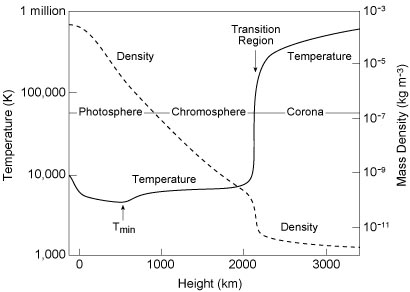
\includegraphics[width=0.95\linewidth]{2023Dundee/Figures/valc.png} \\
%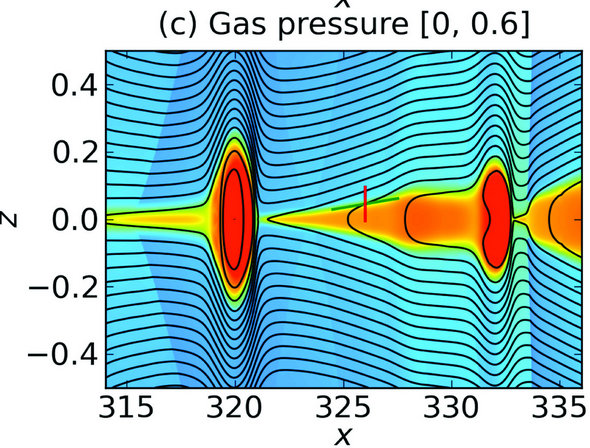
\includegraphics[width=0.95\linewidth]{2023RAS/Figures/shibyama.png}
%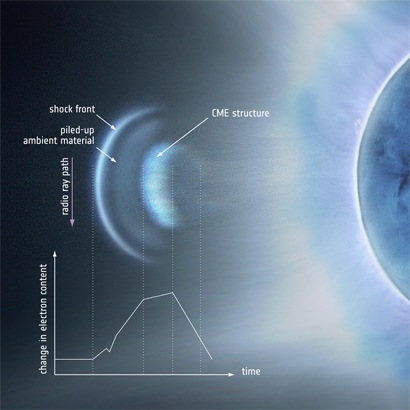
\includegraphics[width=0.32\linewidth]{Figures/cmesketch.jpg}
\end{column}
\end{columns}
\end{frame}

% \begin{frame}{Energy mechanisms}
% \centering
% 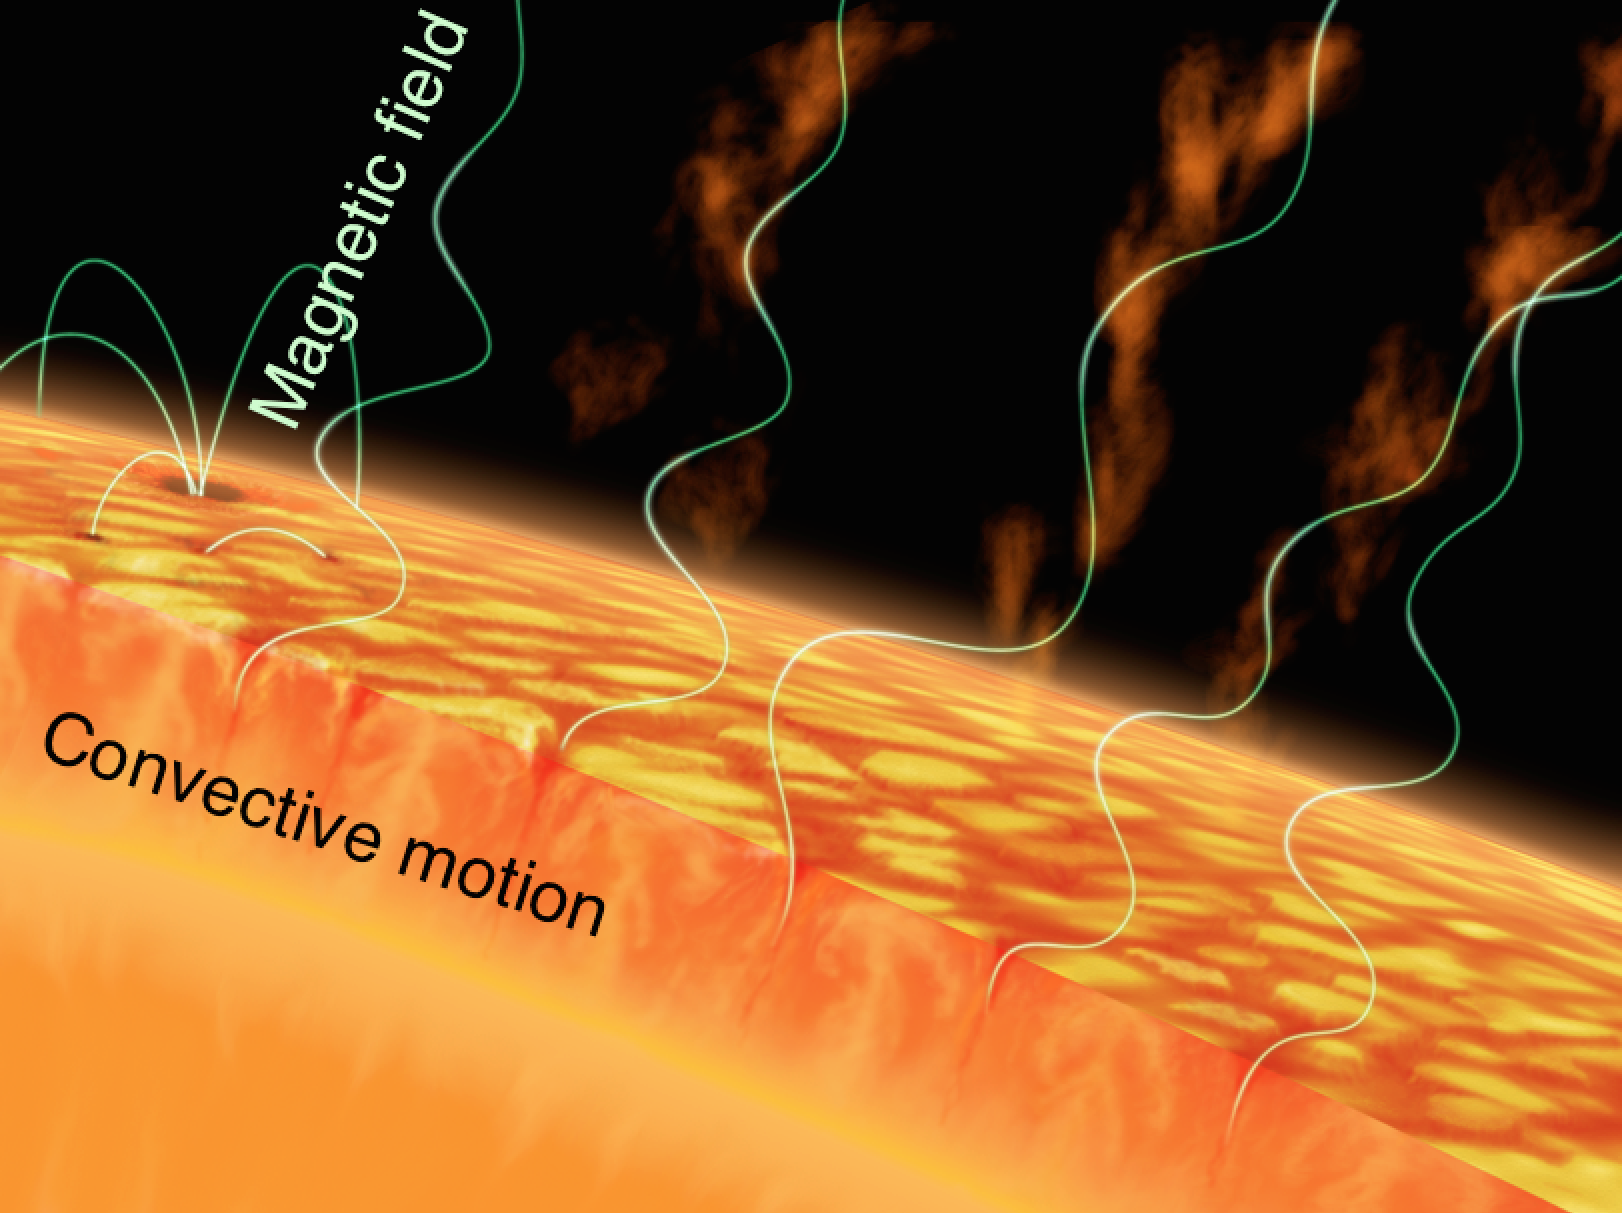
\includegraphics[width=0.45\linewidth]{2023Dundee/Figures/waveheating.png} 
% 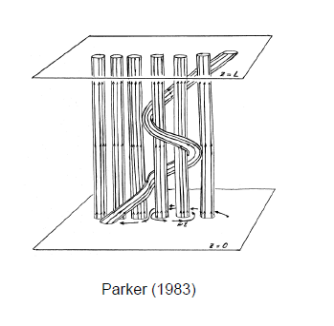
\includegraphics[width=0.45\linewidth,clip=true,trim=0.0cm 1.0cm 0.0cm 0.0cm]{2023Dundee/Figures/reconnection.png}
% \begin{itemize}
%     \item Main methods for converting magnetic energy into thermal energy are broadly categorised as AC (waves) and DC (reconnection)
%     \item Both can feature shocks.
% %    \item Substructure possible.
% \end{itemize}
% \end{frame}

%%%%%%%%%%%%%%%%%%%%%%%%%%%%%%%%%%%%

\begin{frame}{Shocks in plasma}
\begin{columns}
\begin{column}{0.5\textwidth}
\begin{itemize}
    \item Sharp jump in properties across a shock - adiabatic heating (through compression) and dissipative heating (e.g., viscous or resistive)
    \item Wave-driven shocks, e.g., umbral flashes
    \item Impulsively driven shocks - Magnetic reconnection.
%    \item Shocks are common features of magnetic reconnection (Petschek1964, Shibyama+2015).
    \item Chromosphere is partially ionised - ions and neutrals follow different equations.
    \item Two-fluid shocks not well understood.
\end{itemize}
\end{column}
\begin{column}{0.5\textwidth}
%\includegraphics[width=0.32\linewidth]{Figures/Crab_Nebula.jpeg}
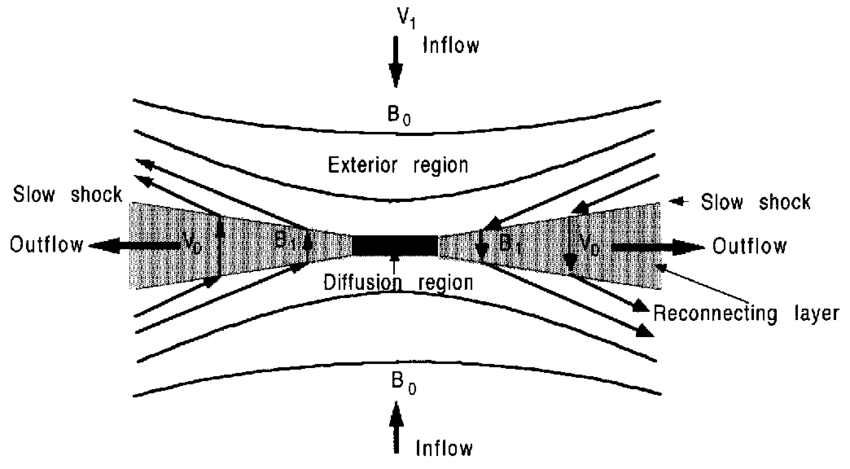
\includegraphics[width=0.95\linewidth]{2023RAS/Figures/petschek.png} \\
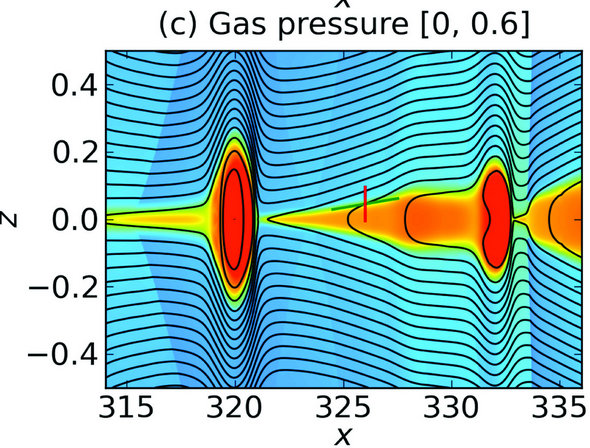
\includegraphics[width=0.95\linewidth]{2023RAS/Figures/shibyama.png}
%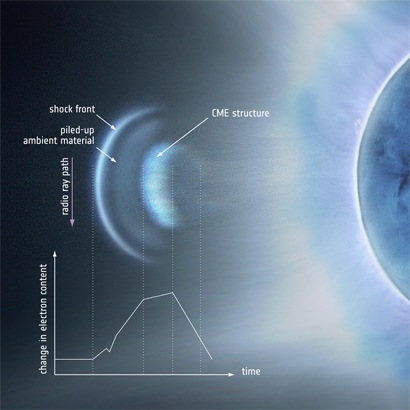
\includegraphics[width=0.32\linewidth]{Figures/cmesketch.jpg}
\end{column}
\end{columns}
\end{frame}

\begin{frame}{Partially ionised chromosphere}
\begin{columns}
\begin{column}{0.5\textwidth}
\begin{itemize}
    \item Chromosphere is partially ionised - ions and neutrals follow different equations.
    \item Partial ionisation known to speed up magnetic reconnection, dissipative heating of Alfven waves, affect stability of systems (KHI, RT, corrugation)
    \item Two-fluid shocks not well understood - high frequency events lead to localised decoupling of ions and neutrals
    \item Missing physics: ionisation/recombination rates increased in shocks, multiple excited neutral hydrogen states, non-equilibrium ionisation, ionisation/excitation cooling, recombination/de-excitation heating..... 
\end{itemize}
\end{column}
\begin{column}{0.5\textwidth}
\includegraphics[width=0.9\linewidth]{Figures/saha2_plot.png} \\
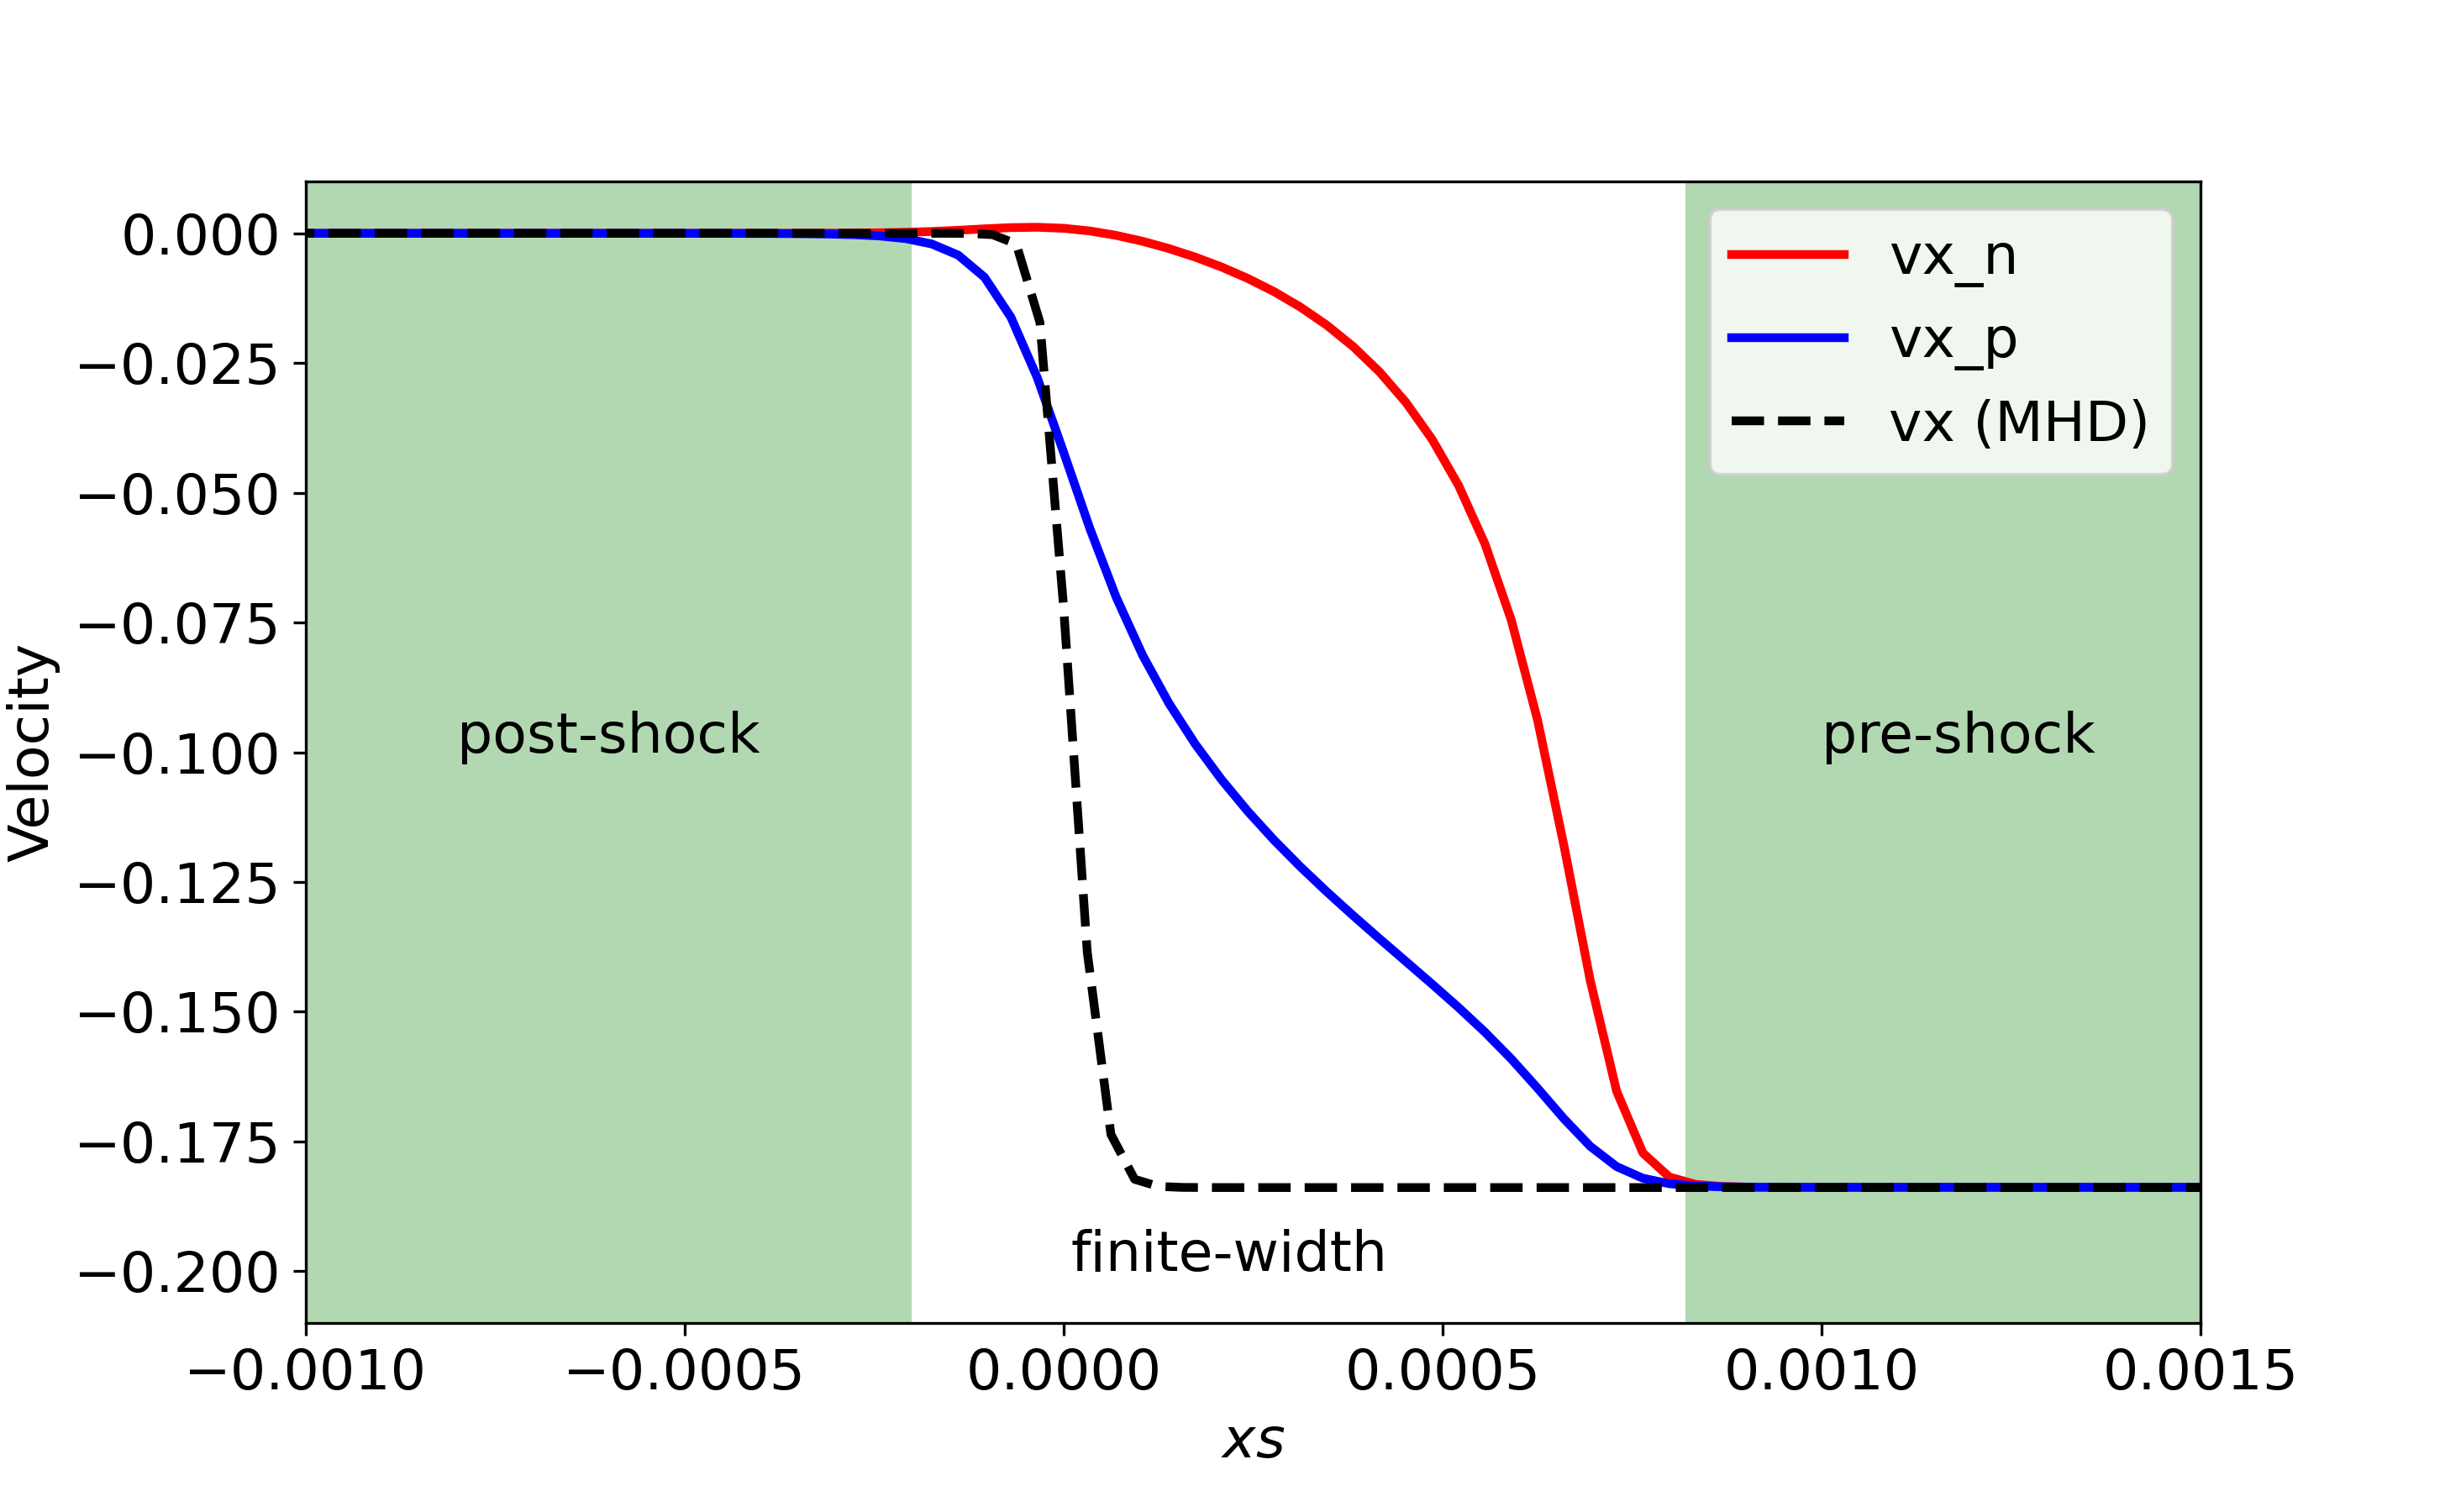
\includegraphics[width=0.95\linewidth]{2023RAS/Figures/shocksub_col.png} \\
%Conservative equations (e.g., two-fluid with thermal collisions) leads to MHD shock jumps, Snow \& Hillier 2019.
\end{column}
\end{columns}
\end{frame}

% \begin{frame}{Two-fluid shocks - overview}
% \begin{columns}
% \begin{column}{0.4\textwidth}
% \begin{itemize}
%     % \item Solar chromosphere is partially ionised.
%     % \item Understanding two-fluid shocks is fundamental to understanding energy transfer and heating in the solar chromosphere and corona.
%     \item Two-fluid shocks have a finite width as opposed to the discontinuous single-fluid MHD case.
%     \item Same overall shock jump but substructure exists.
%     \item Ionisation/recombination rates increased in shocks - needs to be considered.
%     \item Multiple excited neutral hydrogen states, non-equilibrium ionisation, ionisation/excitation cooling, recombination/de-excitation heating..... 
% %    \item Substructure possible.
% \end{itemize}
% %\includegraphics[width=1.0\textwidth,clip=true,trim=1.0cm 1.0cm 1.0cm 1.0cm]{obs_shockloc_contour.png}
% \end{column}
% \begin{column}{0.6\textwidth}
% %\includegraphics[width=0.95\linewidth,clip=true,trim=0.9cm 7.8cm 1.5cm 7.8cm]{poster_comp.pdf} \\
% 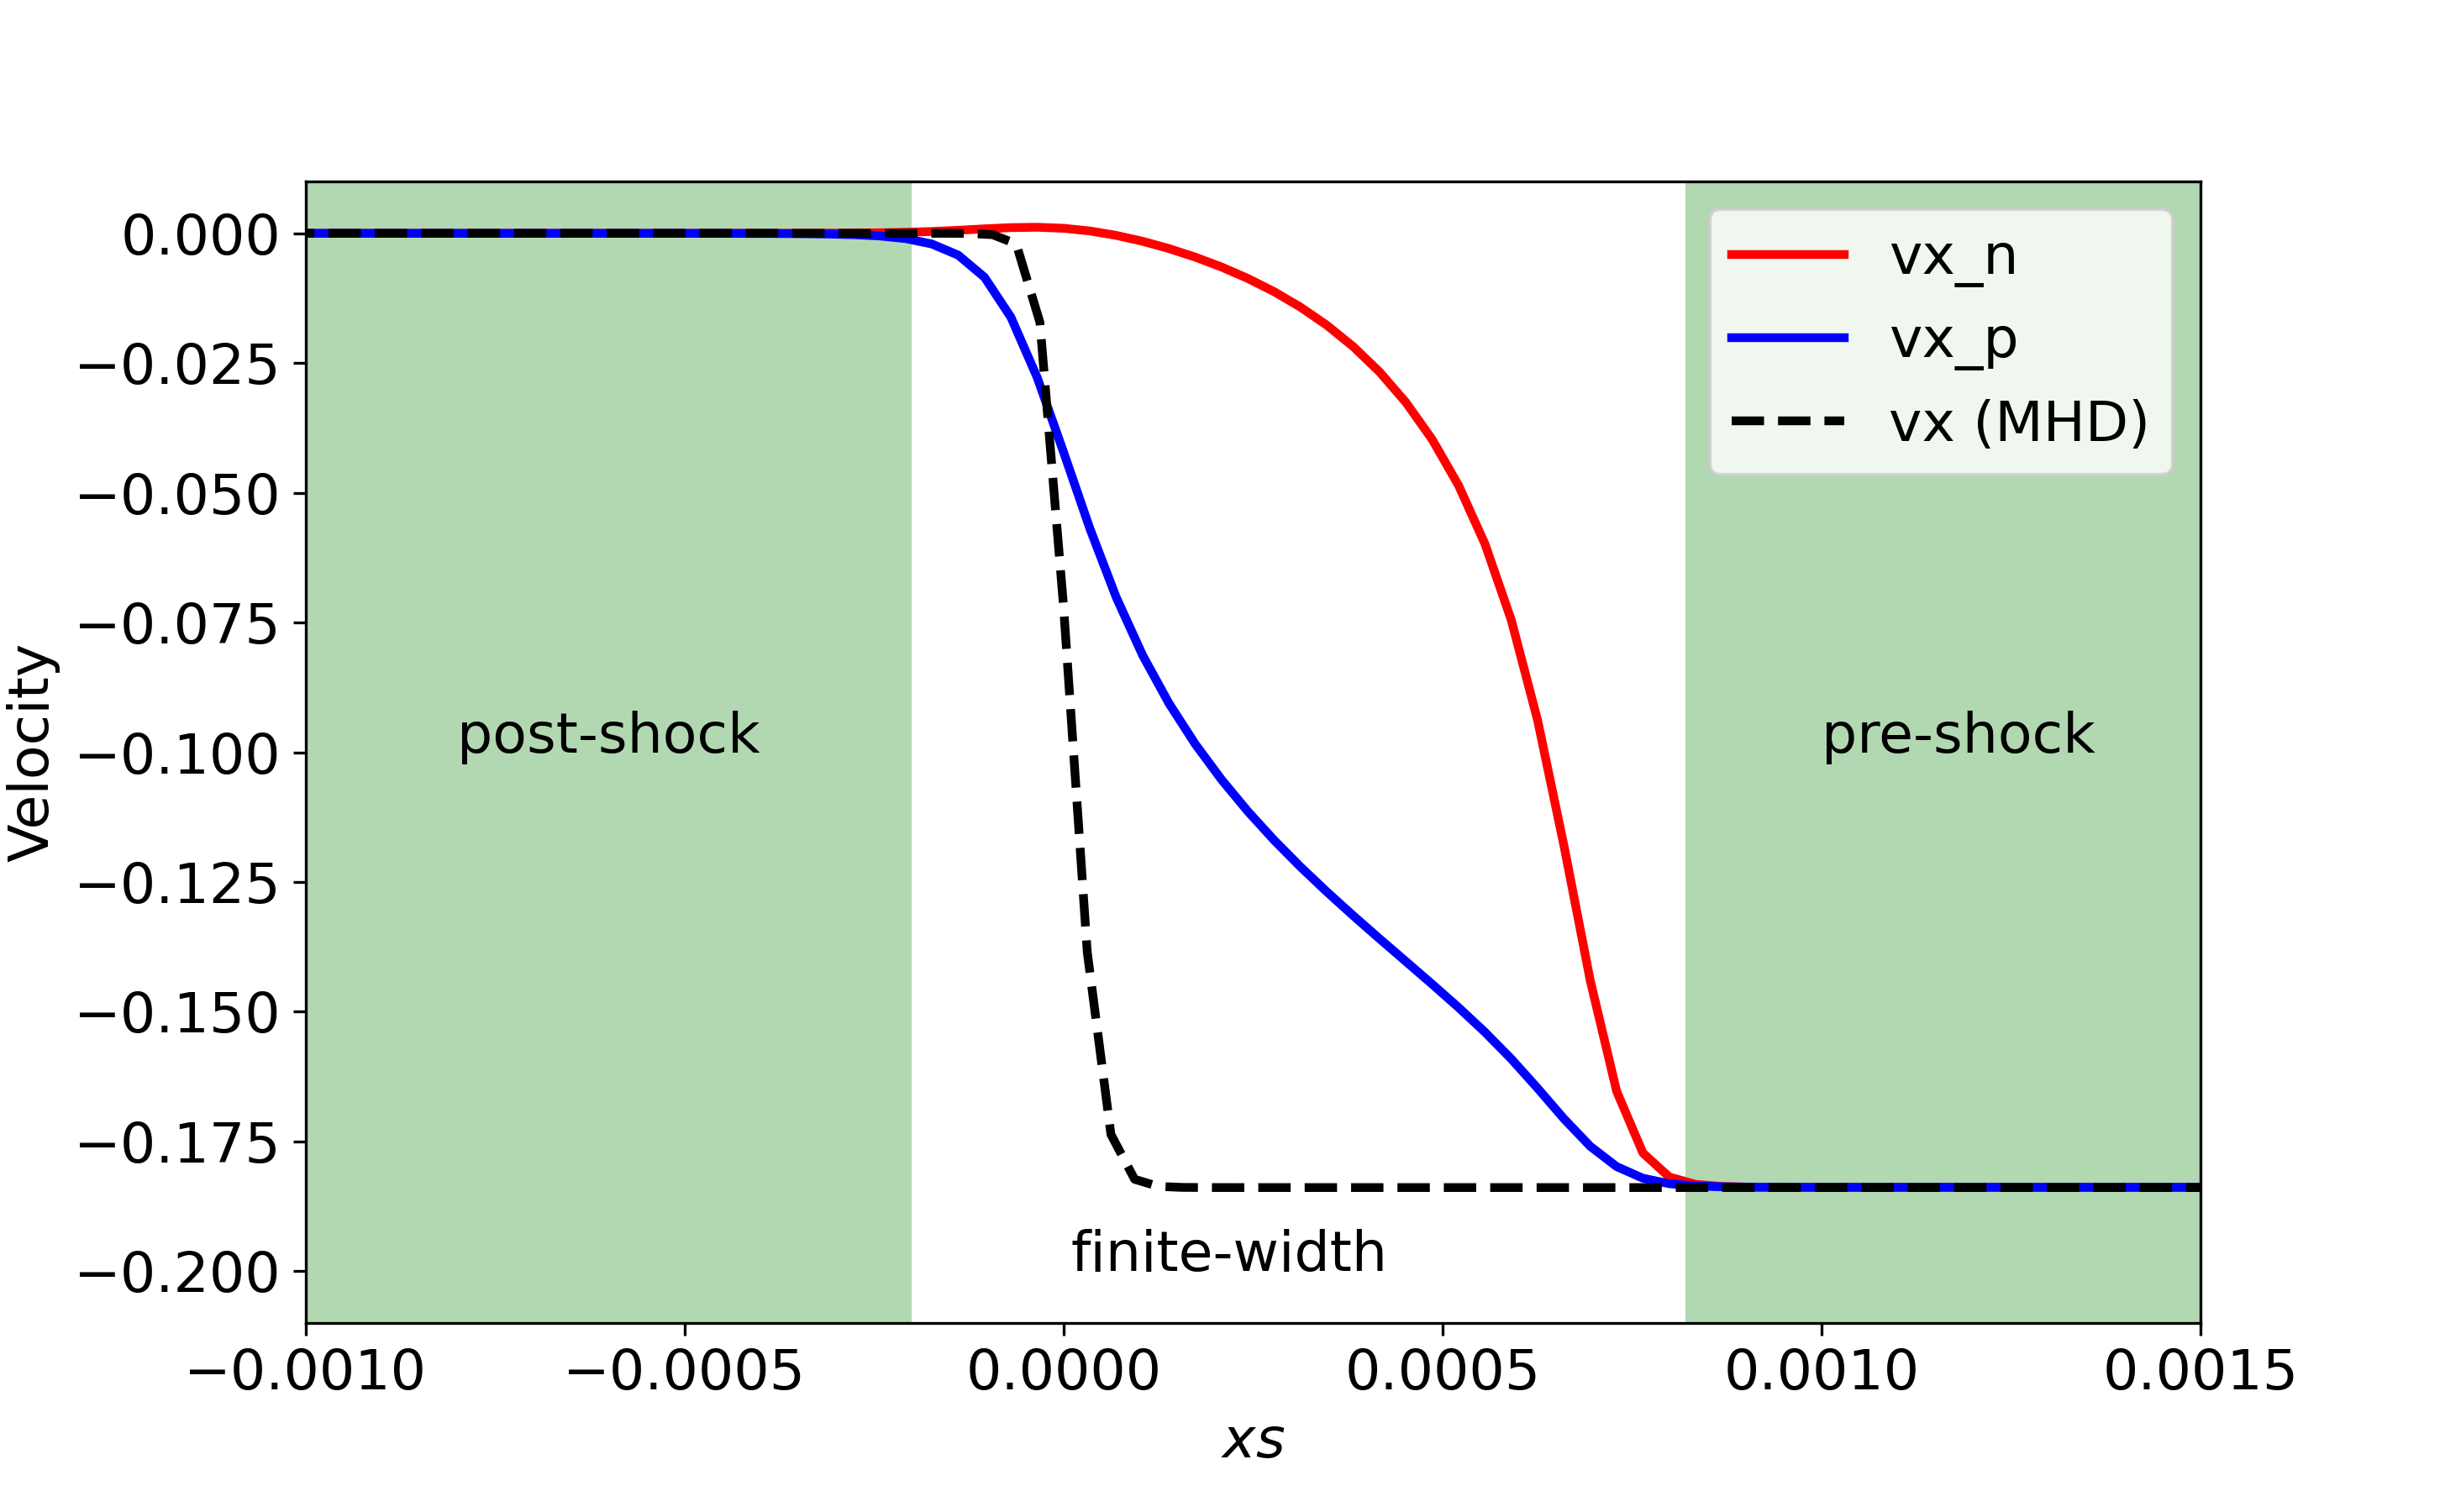
\includegraphics[width=0.95\linewidth]{2023RAS/Figures/shocksub_col.png} \\
% Conservative equations (e.g., two-fluid with thermal collisions) leads to MHD shock jumps, Snow \& Hillier 2019.
% \end{column}
% \end{columns}
% \end{frame}

\begin{frame}{Scientific motivation}
\begin{itemize}
    \item How do partially-ionised effects contribute to heating of solar plasma (and more generally)?
    \item Developed tools to numerically study partially-ionised plasmas.
    \item Analytical methods
    \item Multiple-level, non-equilibrium hydrogen model for ionisation/recombination using collsional/radiative rates in two-fluid framework.
    \item Study how the temperature changes across a partially ionised shock.
    \item See how the temperature jump varies with atmospheric height.
\end{itemize}
\end{frame}

%%%%%%%%%%%%%%%%%%%%%%%%%%%%%%%%%%%%%%%%%%%%%%%%%%%%%%%%%%%%%%%%%%%%%%%%%%%%%%%%%%

\begin{frame}{Ionisation, recombination and ionisation potential in two-fluid shocks}
\footnotesize
\begin{gather}
\frac{\partial \rho _{\text{n}}}{\partial t} + \nabla \cdot (\rho _{\text{n}} \textbf{v}_{\text{n}})= \Gamma _{rec} \rho _{\rm p} - \Gamma _{ion} \rho _{\rm n}, \label{eqn:neutral1}\tag{5} \\
\frac{\partial}{\partial t}(\rho _{\text{n}} \textbf{v}_{\text{n}}) + \nabla \cdot (\rho _{\text{n}} \textbf{v}_{\text{n}} \textbf{v}_{\text{n}} + P_{\text{n}} \textbf{I}) = -\alpha _c \rho_{\text{n}} \rho_{\text{p}} (\textbf{v}_{\text{n}}-\textbf{v}_{\text{p}}) + \Gamma _{rec} \rho _{\rm p} \textbf{v}_{\rm p} - \Gamma _{ion} \rho_{\rm n} \textbf{v}_{\rm n}, \tag{6}\\
\frac{\partial e_{\text{n}}}{\partial t} + \nabla \cdot \left[\textbf{v}_{\text{n}} (e_{\text{n}} +P_{\text{n}}) \right] = -\alpha _c \rho _{\text{n}} \rho _{\text{p}} \left[ \frac{1}{2} (\textbf{v}_{\text{n}} ^2 - \textbf{v}_{\text{p}} ^2)+ \frac{1}{\gamma -1} \left(\frac{P_{\rm n}}{\rho_{\rm n}}-\frac{1}{2}\frac{P_{\rm p}}{\rho_{\rm p}}\right) \right] \nonumber \\ \hspace{0.5cm}+ \frac{1}{2} \left( \Gamma _{rec} \rho _{\rm p} \textbf{v}_{\rm p} ^2 - \Gamma _{ion} \rho _{\rm n} \textbf{v}_{\rm n} ^2 \right) +\frac{1}{ (\gamma-1)} \left( \frac{1}{2} \Gamma _{rec} P_{\rm p} -\Gamma _{ion} P_{\rm n} \right), \tag{7}\\
%e_{\text{n}} = \frac{P_{\text{n}}}{\gamma -1} + \frac{1}{2} \rho _{\text{n}} v_{\text{n}} ^2, \label{eqn:neutral2} \\
\frac{\partial \rho _{\text{p}}}{\partial t} + \nabla \cdot (\rho_{\text{p}} \textbf{v}_{\text{p}}) = - \Gamma _{rec} \rho _{\rm p} + \Gamma _{ion} \rho _{\rm n} \label{eqn:plasma1}\tag{8}\\
\frac{\partial}{\partial t} (\rho_{\text{p}} \textbf{v}_{\text{p}})+ \nabla \cdot \left( \rho_{\text{p}} \textbf{v}_{\text{p}} \textbf{v}_{\text{p}} + P_{\text{p}} \textbf{I} - \textbf{B B} + \frac{\textbf{B}^2}{2} \textbf{I} \right) = \alpha _c \rho_{\text{n}} \rho_{\text{p}}(\textbf{v}_{\text{n}} - \textbf{v}_{\text{p}}) - \Gamma _{rec} \rho _{\rm p} \textbf{v}_{\rm p} + \Gamma _{ion} \rho_{\rm n} \textbf{v}_{\rm n},\tag{9}\\
\frac{\partial}{\partial t} \left( e_{\text{p}} + \frac{\textbf{B}^2}{2} \right) + \nabla \cdot \left[ \textbf{v}_{\text{p}} ( e_{\text{p}} + P_{\text{p}}) -  (\textbf{v}_{\rm p} \times \textbf{B}) \times \textbf{B} \right]  =  \alpha _c \rho _{\text{n}} \rho _{\text{p}} \left[ \frac{1}{2} (\textbf{v}_{\text{n}} ^2 - \textbf{v}_{\text{p}} ^2)+ \frac{1}{\gamma -1} \left(\frac{P_{\rm n}}{\rho_{\rm n}}-\frac{1}{2}\frac{P_{\rm p}}{\rho_{\rm p}}\right) \right] \nonumber \\ \hspace{0.5cm}- \frac{1}{2} \left( \Gamma _{rec} \rho _{\rm p} \textbf{v}_{\rm p} ^2 - \Gamma _{ion} \rho _{\rm n} \textbf{v}_{\rm n} ^2 \right) {- \phi_I + \phi_{heat}} -\frac{1}{ (\gamma-1)} \left( \frac{1}{2} \Gamma _{rec} P_{\rm p} -\Gamma _{ion} P_{\rm n} \right), \label{eqn:ep}\tag{10} \\
\frac{\partial \textbf{B}}{\partial t} - \nabla \times (\textbf{v}_{\text{p}} \times \textbf{B}) = 0.\tag{11}
%e_{\text{p}} = \frac{P_{\text{p}}}{\gamma -1} + \frac{1}{2} \rho _{\text{p}} v_{\text{p}} ^2, \\
%\nabla \cdot \textbf{B} = 0,\label{eqn:plasma2}
\end{gather}
\end{frame}

\begin{frame}{Ionisation, recombination and ionisation potential in two-fluid shocks}
\vspace{-0.5cm}
\footnotesize
\begin{gather}
\mathcolorbox{VioletRed}{\frac{\partial \rho _{\text{n}}}{\partial t} + \nabla \cdot (\rho _{\text{n}} \textbf{v}_{\text{n}})}= \Gamma _{rec} \rho _{\rm p} - \Gamma _{ion} \rho _{\rm n}, \label{eqn:neutral1}\tag{5} \\
\mathcolorbox{VioletRed}{\frac{\partial}{\partial t}(\rho _{\text{n}} \textbf{v}_{\text{n}}) + \nabla \cdot (\rho _{\text{n}} \textbf{v}_{\text{n}} \textbf{v}_{\text{n}} + P_{\text{n}} \textbf{I})} = -\alpha _c \rho_{\text{n}} \rho_{\text{p}} (\textbf{v}_{\text{n}}-\textbf{v}_{\text{p}}) + \Gamma _{rec} \rho _{\rm p} \textbf{v}_{\rm p} - \Gamma _{ion} \rho_{\rm n} \textbf{v}_{\rm n}, \tag{6}\\
\mathcolorbox{VioletRed}{\frac{\partial e_{\text{n}}}{\partial t} + \nabla \cdot \left[\textbf{v}_{\text{n}} (e_{\text{n}} +P_{\text{n}}) \right]} = -\alpha _c \rho _{\text{n}} \rho _{\text{p}} \left[ \frac{1}{2} (\textbf{v}_{\text{n}} ^2 - \textbf{v}_{\text{p}} ^2)+ \frac{1}{\gamma -1} \left(\frac{P_{\rm n}}{\rho_{\rm n}}-\frac{1}{2}\frac{P_{\rm p}}{\rho_{\rm p}}\right) \right] \nonumber \\ \hspace{0.5cm}+ \frac{1}{2} \left( \Gamma _{rec} \rho _{\rm p} \textbf{v}_{\rm p} ^2 - \Gamma _{ion} \rho _{\rm n} \textbf{v}_{\rm n} ^2 \right) +\frac{1}{ (\gamma-1)} \left( \frac{1}{2} \Gamma _{rec} P_{\rm p} -\Gamma _{ion} P_{\rm n} \right), \tag{7}\\
%e_{\text{n}} = \frac{P_{\text{n}}}{\gamma -1} + \frac{1}{2} \rho _{\text{n}} v_{\text{n}} ^2, \label{eqn:neutral2} \\
\frac{\partial \rho _{\text{p}}}{\partial t} + \nabla \cdot (\rho_{\text{p}} \textbf{v}_{\text{p}}) = - \Gamma _{rec} \rho _{\rm p} + \Gamma _{ion} \rho _{\rm n} \label{eqn:plasma1}\tag{8}\\
\frac{\partial}{\partial t} (\rho_{\text{p}} \textbf{v}_{\text{p}})+ \nabla \cdot \left( \rho_{\text{p}} \textbf{v}_{\text{p}} \textbf{v}_{\text{p}} + P_{\text{p}} \textbf{I} - \textbf{B B} + \frac{\textbf{B}^2}{2} \textbf{I} \right) = \alpha _c \rho_{\text{n}} \rho_{\text{p}}(\textbf{v}_{\text{n}} - \textbf{v}_{\text{p}}) - \Gamma _{rec} \rho _{\rm p} \textbf{v}_{\rm p} + \Gamma _{ion} \rho_{\rm n} \textbf{v}_{\rm n},\tag{9}\\
\frac{\partial}{\partial t} \left( e_{\text{p}} + \frac{\textbf{B}^2}{2} \right) + \nabla \cdot \left[ \textbf{v}_{\text{p}} ( e_{\text{p}} + P_{\text{p}}) -  (\textbf{v}_{\rm p} \times \textbf{B}) \times \textbf{B} \right]  =  \alpha _c \rho _{\text{n}} \rho _{\text{p}} \left[ \frac{1}{2} (\textbf{v}_{\text{n}} ^2 - \textbf{v}_{\text{p}} ^2)+ \frac{1}{\gamma -1} \left(\frac{P_{\rm n}}{\rho_{\rm n}}-\frac{1}{2}\frac{P_{\rm p}}{\rho_{\rm p}}\right) \right] \nonumber \\ \hspace{0.5cm}- \frac{1}{2} \left( \Gamma _{rec} \rho _{\rm p} \textbf{v}_{\rm p} ^2 - \Gamma _{ion} \rho _{\rm n} \textbf{v}_{\rm n} ^2 \right) {- \phi_I + \phi_{heat}} -\frac{1}{ (\gamma-1)} \left( \frac{1}{2} \Gamma _{rec} P_{\rm p} -\Gamma _{ion} P_{\rm n} \right), \label{eqn:ep} \tag{10}\\
\frac{\partial \textbf{B}}{\partial t} - \nabla \times (\textbf{v}_{\text{p}} \times \textbf{B}) = 0.\tag{11}
%e_{\text{p}} = \frac{P_{\text{p}}}{\gamma -1} + \frac{1}{2} \rho _{\text{p}} v_{\text{p}} ^2, \\
%\nabla \cdot \textbf{B} = 0,\label{eqn:plasma2}
\end{gather}
\end{frame}

\begin{frame}{Ionisation, recombination and ionisation potential in two-fluid shocks}
\vspace{-0.5cm}
\footnotesize
\begin{gather}
\frac{\partial \rho _{\text{n}}}{\partial t} + \nabla \cdot (\rho _{\text{n}} \textbf{v}_{\text{n}})= \Gamma _{rec} \rho _{\rm p} - \Gamma _{ion} \rho _{\rm n}, \label{eqn:neutral1}\tag{5} \\
\frac{\partial}{\partial t}(\rho _{\text{n}} \textbf{v}_{\text{n}}) + \nabla \cdot (\rho _{\text{n}} \textbf{v}_{\text{n}} \textbf{v}_{\text{n}} + P_{\text{n}} \textbf{I}) = -\alpha _c \rho_{\text{n}} \rho_{\text{p}} (\textbf{v}_{\text{n}}-\textbf{v}_{\text{p}}) + \Gamma _{rec} \rho _{\rm p} \textbf{v}_{\rm p} - \Gamma _{ion} \rho_{\rm n} \textbf{v}_{\rm n}, \tag{6}\\
\frac{\partial e_{\text{n}}}{\partial t} + \nabla \cdot \left[\textbf{v}_{\text{n}} (e_{\text{n}} +P_{\text{n}}) \right] = -\alpha _c \rho _{\text{n}} \rho _{\text{p}} \left[ \frac{1}{2} (\textbf{v}_{\text{n}} ^2 - \textbf{v}_{\text{p}} ^2)+ \frac{1}{\gamma -1} \left(\frac{P_{\rm n}}{\rho_{\rm n}}-\frac{1}{2}\frac{P_{\rm p}}{\rho_{\rm p}}\right) \right] \nonumber \\ \hspace{0.5cm}+ \frac{1}{2} \left( \Gamma _{rec} \rho _{\rm p} \textbf{v}_{\rm p} ^2 - \Gamma _{ion} \rho _{\rm n} \textbf{v}_{\rm n} ^2 \right) +\frac{1}{ (\gamma-1)} \left( \frac{1}{2} \Gamma _{rec} P_{\rm p} -\Gamma _{ion} P_{\rm n} \right), \tag{7}\\
%e_{\text{n}} = \frac{P_{\text{n}}}{\gamma -1} + \frac{1}{2} \rho _{\text{n}} v_{\text{n}} ^2, \label{eqn:neutral2} \\
\mathcolorbox{BlueGreen}{\frac{\partial \rho _{\text{p}}}{\partial t} + \nabla \cdot (\rho_{\text{p}} \textbf{v}_{\text{p}})} = - \Gamma _{rec} \rho _{\rm p} + \Gamma _{ion} \rho _{\rm n} \label{eqn:plasma1}\tag{8}\\
\mathcolorbox{BlueGreen}{\frac{\partial}{\partial t} (\rho_{\text{p}} \textbf{v}_{\text{p}})+ \nabla \cdot \left( \rho_{\text{p}} \textbf{v}_{\text{p}} \textbf{v}_{\text{p}} + P_{\text{p}} \textbf{I} - \textbf{B B} + \frac{\textbf{B}^2}{2} \textbf{I} \right)} = \alpha _c \rho_{\text{n}} \rho_{\text{p}}(\textbf{v}_{\text{n}} - \textbf{v}_{\text{p}}) - \Gamma _{rec} \rho _{\rm p} \textbf{v}_{\rm p} + \Gamma _{ion} \rho_{\rm n} \textbf{v}_{\rm n},\tag{9}\\
\mathcolorbox{BlueGreen}{\frac{\partial}{\partial t} \left( e_{\text{p}} + \frac{\textbf{B}^2}{2} \right) + \nabla \cdot \left[ \textbf{v}_{\text{p}} ( e_{\text{p}} + P_{\text{p}}) -  (\textbf{v}_{\rm p} \times \textbf{B}) \times \textbf{B} \right] } =  \alpha _c \rho _{\text{n}} \rho _{\text{p}} \left[ \frac{1}{2} (\textbf{v}_{\text{n}} ^2 - \textbf{v}_{\text{p}} ^2)+ \frac{1}{\gamma -1} \left(\frac{P_{\rm n}}{\rho_{\rm n}}-\frac{1}{2}\frac{P_{\rm p}}{\rho_{\rm p}}\right) \right] \nonumber \\ \hspace{0.5cm}- \frac{1}{2} \left( \Gamma _{rec} \rho _{\rm p} \textbf{v}_{\rm p} ^2 - \Gamma _{ion} \rho _{\rm n} \textbf{v}_{\rm n} ^2 \right) {- \phi_I + \phi_{heat}} -\frac{1}{ (\gamma-1)} \left( \frac{1}{2} \Gamma _{rec} P_{\rm p} -\Gamma _{ion} P_{\rm n} \right), \label{eqn:ep}\tag{10} \\
\mathcolorbox{BlueGreen}{\frac{\partial \textbf{B}}{\partial t} - \nabla \times (\textbf{v}_{\text{p}} \times \textbf{B}) = 0.}\tag{11}
%e_{\text{p}} = \frac{P_{\text{p}}}{\gamma -1} + \frac{1}{2} \rho _{\text{p}} v_{\text{p}} ^2, \\
%\nabla \cdot \textbf{B} = 0,\label{eqn:plasma2}
\end{gather}
\end{frame}

\begin{frame}{Ionisation, recombination and ionisation potential in two-fluid shocks}
\vspace{-0.5cm}
\footnotesize
\begin{gather}
\frac{\partial \rho _{\text{n}}}{\partial t} + \nabla \cdot (\rho _{\text{n}} \textbf{v}_{\text{n}})= \Gamma _{rec} \rho _{\rm p} - \Gamma _{ion} \rho _{\rm n}, \label{eqn:neutral1}\tag{5} \\
\frac{\partial}{\partial t}(\rho _{\text{n}} \textbf{v}_{\text{n}}) + \nabla \cdot (\rho _{\text{n}} \textbf{v}_{\text{n}} \textbf{v}_{\text{n}} + P_{\text{n}} \textbf{I}) =\mathcolorbox{YellowOrange}{ -\alpha _c \rho_{\text{n}} \rho_{\text{p}} (\textbf{v}_{\text{n}}-\textbf{v}_{\text{p}})} + \Gamma _{rec} \rho _{\rm p} \textbf{v}_{\rm p} - \Gamma _{ion} \rho_{\rm n} \textbf{v}_{\rm n}, \tag{6}\\
\frac{\partial e_{\text{n}}}{\partial t} + \nabla \cdot \left[\textbf{v}_{\text{n}} (e_{\text{n}} +P_{\text{n}}) \right] = \mathcolorbox{YellowOrange}{-\alpha _c \rho _{\text{n}} \rho _{\text{p}} \left[ \frac{1}{2} (\textbf{v}_{\text{n}} ^2 - \textbf{v}_{\text{p}} ^2)+ \frac{1}{\gamma -1} \left(\frac{P_{\rm n}}{\rho_{\rm n}}-\frac{1}{2}\frac{P_{\rm p}}{\rho_{\rm p}}\right) \right]} \nonumber \\ \hspace{0.5cm}+ \frac{1}{2} \left( \Gamma _{rec} \rho _{\rm p} \textbf{v}_{\rm p} ^2 - \Gamma _{ion} \rho _{\rm n} \textbf{v}_{\rm n} ^2 \right) +\frac{1}{ (\gamma-1)} \left( \frac{1}{2} \Gamma _{rec} P_{\rm p} -\Gamma _{ion} P_{\rm n} \right), \tag{7}\\
%e_{\text{n}} = \frac{P_{\text{n}}}{\gamma -1} + \frac{1}{2} \rho _{\text{n}} v_{\text{n}} ^2, \label{eqn:neutral2} \\
\frac{\partial \rho _{\text{p}}}{\partial t} + \nabla \cdot (\rho_{\text{p}} \textbf{v}_{\text{p}}) = - \Gamma _{rec} \rho _{\rm p} + \Gamma _{ion} \rho _{\rm n} \label{eqn:plasma1}\tag{8}\\
\frac{\partial}{\partial t} (\rho_{\text{p}} \textbf{v}_{\text{p}})+ \nabla \cdot \left( \rho_{\text{p}} \textbf{v}_{\text{p}} \textbf{v}_{\text{p}} + P_{\text{p}} \textbf{I} - \textbf{B B} + \frac{\textbf{B}^2}{2} \textbf{I} \right) = \mathcolorbox{YellowOrange}{\alpha _c \rho_{\text{n}} \rho_{\text{p}}(\textbf{v}_{\text{n}} - \textbf{v}_{\text{p}})} - \Gamma _{rec} \rho _{\rm p} \textbf{v}_{\rm p} + \Gamma _{ion} \rho_{\rm n} \textbf{v}_{\rm n},\tag{9}\\
\frac{\partial}{\partial t} \left( e_{\text{p}} + \frac{\textbf{B}^2}{2} \right) + \nabla \cdot \left[ \textbf{v}_{\text{p}} ( e_{\text{p}} + P_{\text{p}}) -  (\textbf{v}_{\rm p} \times \textbf{B}) \times \textbf{B} \right]  = \mathcolorbox{YellowOrange}{ \alpha _c \rho _{\text{n}} \rho _{\text{p}} \left[ \frac{1}{2} (\textbf{v}_{\text{n}} ^2 - \textbf{v}_{\text{p}} ^2)+ \frac{1}{\gamma -1} \left(\frac{P_{\rm n}}{\rho_{\rm n}}-\frac{1}{2}\frac{P_{\rm p}}{\rho_{\rm p}}\right) \right]} \nonumber \\ \hspace{0.5cm}- \frac{1}{2} \left( \Gamma _{rec} \rho _{\rm p} \textbf{v}_{\rm p} ^2 - \Gamma _{ion} \rho _{\rm n} \textbf{v}_{\rm n} ^2 \right) {- \phi_I + \phi_{heat}} -\frac{1}{ (\gamma-1)} \left( \frac{1}{2} \Gamma _{rec} P_{\rm p} -\Gamma _{ion} P_{\rm n} \right), \label{eqn:ep} \tag{10}\\
\frac{\partial \textbf{B}}{\partial t} - \nabla \times (\textbf{v}_{\text{p}} \times \textbf{B}) = 0.\tag{11}
%e_{\text{p}} = \frac{P_{\text{p}}}{\gamma -1} + \frac{1}{2} \rho _{\text{p}} v_{\text{p}} ^2, \\
%\nabla \cdot \textbf{B} = 0,\label{eqn:plasma2}
\end{gather}
\end{frame}

\begin{frame}{Ionisation, recombination and ionisation potential in two-fluid shocks}
\vspace{-0.5cm}
\footnotesize
\begin{gather}
\frac{\partial \rho _{\text{n}}}{\partial t} + \nabla \cdot (\rho _{\text{n}} \textbf{v}_{\text{n}})= \mathcolorbox{LimeGreen}{\Gamma _{rec} \rho _{\rm p} - \Gamma _{ion} \rho _{\rm n},} \label{eqn:neutral1}\tag{5} \\
\frac{\partial}{\partial t}(\rho _{\text{n}} \textbf{v}_{\text{n}}) + \nabla \cdot (\rho _{\text{n}} \textbf{v}_{\text{n}} \textbf{v}_{\text{n}} + P_{\text{n}} \textbf{I}) = -\alpha _c \rho_{\text{n}} \rho_{\text{p}} (\textbf{v}_{\text{n}}-\textbf{v}_{\text{p}}) + \mathcolorbox{LimeGreen}{\Gamma _{rec} \rho _{\rm p} \textbf{v}_{\rm p} - \Gamma _{ion} \rho_{\rm n} \textbf{v}_{\rm n}}, \tag{6}\\
\frac{\partial e_{\text{n}}}{\partial t} + \nabla \cdot \left[\textbf{v}_{\text{n}} (e_{\text{n}} +P_{\text{n}}) \right] = -\alpha _c \rho _{\text{n}} \rho _{\text{p}} \left[ \frac{1}{2} (\textbf{v}_{\text{n}} ^2 - \textbf{v}_{\text{p}} ^2)+ \frac{1}{\gamma -1} \left(\frac{P_{\rm n}}{\rho_{\rm n}}-\frac{1}{2}\frac{P_{\rm p}}{\rho_{\rm p}}\right) \right] \nonumber \\ \hspace{0.5cm}+ \mathcolorbox{LimeGreen}{\frac{1}{2} \left( \Gamma _{rec} \rho _{\rm p} \textbf{v}_{\rm p} ^2 - \Gamma _{ion} \rho _{\rm n} \textbf{v}_{\rm n} ^2 \right) +\frac{1}{ (\gamma-1)} \left( \frac{1}{2} \Gamma _{rec} P_{\rm p} -\Gamma _{ion} P_{\rm n} \right),} \tag{7}\\
%e_{\text{n}} = \frac{P_{\text{n}}}{\gamma -1} + \frac{1}{2} \rho _{\text{n}} v_{\text{n}} ^2, \label{eqn:neutral2} \\
\frac{\partial \rho _{\text{p}}}{\partial t} + \nabla \cdot (\rho_{\text{p}} \textbf{v}_{\text{p}}) = \mathcolorbox{LimeGreen}{- \Gamma _{rec} \rho _{\rm p} + \Gamma _{ion} \rho _{\rm n}} \label{eqn:plasma1}\tag{8}\\
\frac{\partial}{\partial t} (\rho_{\text{p}} \textbf{v}_{\text{p}})+ \nabla \cdot \left( \rho_{\text{p}} \textbf{v}_{\text{p}} \textbf{v}_{\text{p}} + P_{\text{p}} \textbf{I} - \textbf{B B} + \frac{\textbf{B}^2}{2} \textbf{I} \right) = \alpha _c \rho_{\text{n}} \rho_{\text{p}}(\textbf{v}_{\text{n}} - \textbf{v}_{\text{p}}) \mathcolorbox{LimeGreen}{- \Gamma _{rec} \rho _{\rm p} \textbf{v}_{\rm p} + \Gamma _{ion} \rho_{\rm n} \textbf{v}_{\rm n},}\tag{9}\\
\frac{\partial}{\partial t} \left( e_{\text{p}} + \frac{\textbf{B}^2}{2} \right) + \nabla \cdot \left[ \textbf{v}_{\text{p}} ( e_{\text{p}} + P_{\text{p}}) -  (\textbf{v}_{\rm p} \times \textbf{B}) \times \textbf{B} \right]  =  \alpha _c \rho _{\text{n}} \rho _{\text{p}} \left[ \frac{1}{2} (\textbf{v}_{\text{n}} ^2 - \textbf{v}_{\text{p}} ^2)+ \frac{1}{\gamma -1} \left(\frac{P_{\rm n}}{\rho_{\rm n}}-\frac{1}{2}\frac{P_{\rm p}}{\rho_{\rm p}}\right) \right] \nonumber \\ \hspace{0.5cm}\mathcolorbox{LimeGreen}{- \frac{1}{2} \left( \Gamma _{rec} \rho _{\rm p} \textbf{v}_{\rm p} ^2 - \Gamma _{ion} \rho _{\rm n} \textbf{v}_{\rm n} ^2 \right)} {- \phi_I + \phi_{heat}} \mathcolorbox{LimeGreen}{-\frac{1}{ (\gamma-1)} \left( \frac{1}{2} \Gamma _{rec} P_{\rm p} -\Gamma _{ion} P_{\rm n} \right)}, \label{eqn:ep} \tag{10}\\
\frac{\partial \textbf{B}}{\partial t} - \nabla \times (\textbf{v}_{\text{p}} \times \textbf{B}) = 0.\tag{11}
%e_{\text{p}} = \frac{P_{\text{p}}}{\gamma -1} + \frac{1}{2} \rho _{\text{p}} v_{\text{p}} ^2, \\
%\nabla \cdot \textbf{B} = 0,\label{eqn:plasma2}
\end{gather}
\end{frame}

\begin{frame}{Ionisation process}
\begin{columns}
\begin{column}{0.4\textwidth}
\begin{itemize}
    % \item Solar chromosphere is partially ionised.
    % \item Understanding two-fluid shocks is fundamental to understanding energy transfer and heating in the solar chromosphere and corona.
    \item Ionisation is a three-body process
    \item Free electron deposits energy to release bound electron
    \item Net loss of energy from the plasma during ionisation
%    \item Substructure possible.
\end{itemize}
%\includegraphics[width=1.0\textwidth,clip=true,trim=1.0cm 1.0cm 1.0cm 1.0cm]{obs_shockloc_contour.png}
\end{column}
\begin{column}{0.6\textwidth}
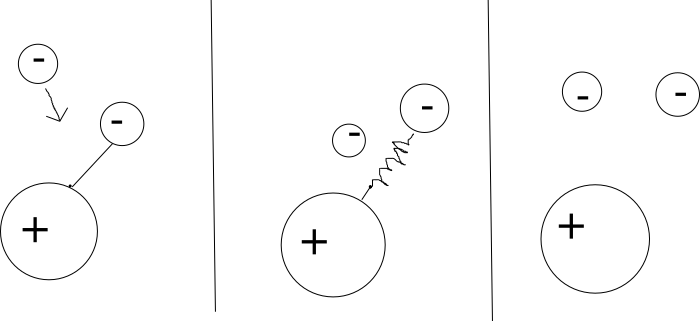
\includegraphics[width=0.95\linewidth]{Figures/hydrogensketchion.png} 
\end{column}
\end{columns}
\end{frame}

\begin{frame}{Ionisation, recombination and ionisation potential in two-fluid shocks}
\footnotesize
\begin{gather}
\frac{\partial \rho _{\text{n}}}{\partial t} + \nabla \cdot (\rho _{\text{n}} \textbf{v}_{\text{n}})= \Gamma _{rec} \rho _{\rm p} - \Gamma _{ion} \rho _{\rm n}, \label{eqn:neutral1}\tag{5} \\
\frac{\partial}{\partial t}(\rho _{\text{n}} \textbf{v}_{\text{n}}) + \nabla \cdot (\rho _{\text{n}} \textbf{v}_{\text{n}} \textbf{v}_{\text{n}} + P_{\text{n}} \textbf{I}) = -\alpha _c \rho_{\text{n}} \rho_{\text{p}} (\textbf{v}_{\text{n}}-\textbf{v}_{\text{p}}) + \Gamma _{rec} \rho _{\rm p} \textbf{v}_{\rm p} - \Gamma _{ion} \rho_{\rm n} \textbf{v}_{\rm n},\tag{6} \\
\frac{\partial e_{\text{n}}}{\partial t} + \nabla \cdot \left[\textbf{v}_{\text{n}} (e_{\text{n}} +P_{\text{n}}) \right] = -\alpha _c \rho _{\text{n}} \rho _{\text{p}} \left[ \frac{1}{2} (\textbf{v}_{\text{n}} ^2 - \textbf{v}_{\text{p}} ^2)+ \frac{1}{\gamma -1} \left(\frac{P_{\rm n}}{\rho_{\rm n}}-\frac{1}{2}\frac{P_{\rm p}}{\rho_{\rm p}}\right) \right] \nonumber \\ \hspace{0.5cm}+ \frac{1}{2} \left( \Gamma _{rec} \rho _{\rm p} \textbf{v}_{\rm p} ^2 - \Gamma _{ion} \rho _{\rm n} \textbf{v}_{\rm n} ^2 \right) +\frac{1}{ (\gamma-1)} \left( \frac{1}{2} \Gamma _{rec} P_{\rm p} -\Gamma _{ion} P_{\rm n} \right), \tag{7}\\
%e_{\text{n}} = \frac{P_{\text{n}}}{\gamma -1} + \frac{1}{2} \rho _{\text{n}} v_{\text{n}} ^2, \label{eqn:neutral2} \\
\frac{\partial \rho _{\text{p}}}{\partial t} + \nabla \cdot (\rho_{\text{p}} \textbf{v}_{\text{p}}) = - \Gamma _{rec} \rho _{\rm p} + \Gamma _{ion} \rho _{\rm n} \label{eqn:plasma1}\tag{8}\\
\frac{\partial}{\partial t} (\rho_{\text{p}} \textbf{v}_{\text{p}})+ \nabla \cdot \left( \rho_{\text{p}} \textbf{v}_{\text{p}} \textbf{v}_{\text{p}} + P_{\text{p}} \textbf{I} - \textbf{B B} + \frac{\textbf{B}^2}{2} \textbf{I} \right) = \alpha _c \rho_{\text{n}} \rho_{\text{p}}(\textbf{v}_{\text{n}} - \textbf{v}_{\text{p}}) - \Gamma _{rec} \rho _{\rm p} \textbf{v}_{\rm p} + \Gamma _{ion} \rho_{\rm n} \textbf{v}_{\rm n},\tag{9}\\
\frac{\partial}{\partial t} \left( e_{\text{p}} + \frac{\textbf{B}^2}{2} \right) + \nabla \cdot \left[ \textbf{v}_{\text{p}} ( e_{\text{p}} + P_{\text{p}}) -  (\textbf{v}_{\rm p} \times \textbf{B}) \times \textbf{B} \right]  =  \alpha _c \rho _{\text{n}} \rho _{\text{p}} \left[ \frac{1}{2} (\textbf{v}_{\text{n}} ^2 - \textbf{v}_{\text{p}} ^2)+ \frac{1}{\gamma -1} \left(\frac{P_{\rm n}}{\rho_{\rm n}}-\frac{1}{2}\frac{P_{\rm p}}{\rho_{\rm p}}\right) \right] \nonumber \\ \hspace{0.5cm}- \frac{1}{2} \left( \Gamma _{rec} \rho _{\rm p} \textbf{v}_{\rm p} ^2 - \Gamma _{ion} \rho _{\rm n} \textbf{v}_{\rm n} ^2 \right) \mathcolorbox{yellow}{- \phi_I + \phi_{heat}} -\frac{1}{ (\gamma-1)} \left( \frac{1}{2} \Gamma _{rec} P_{\rm p} -\Gamma _{ion} P_{\rm n} \right), \label{eqn:ep} \tag{10}\\
\frac{\partial \textbf{B}}{\partial t} - \nabla \times (\textbf{v}_{\text{p}} \times \textbf{B}) = 0.\tag{11}
%e_{\text{p}} = \frac{P_{\text{p}}}{\gamma -1} + \frac{1}{2} \rho _{\text{p}} v_{\text{p}} ^2, \\
%\nabla \cdot \textbf{B} = 0,\label{eqn:plasma2}
\end{gather}
\end{frame}

%%%%%%%%%%%%%%%%%%%%%%%%%%%%%%%%%%%%%%%%%%%%%%%%%%%%%%%%%%%%%%%%%
% \begin{frame}{Analytical solutions}
% \begin{columns}
% \begin{column}{0.4\textwidth}
% \begin{itemize}
% %\item Two-fluid model - ion+electron plasma, and bulk neutral fluid.
% \item Shocks are approximately 1D - allows analytical solutions to exist.
% \item Sufficient far from a shock, the species are coupled in terms of velocity
% \item In the absence of loss/heat terms, reduces to MHD
% \end{itemize}
% \end{column}
% \begin{column}{0.6\textwidth}
% \end{column}
% \end{columns}
% \end{frame}

% \begin{frame}{IRIP shock jumps}
% \textbf{Ionisation recombination and ionisation potential}
% \begin{gather}
% \nabla \cdot (\rho _{\text{n}} \textbf{v}_{\text{p}})= S_{mass}, \\
% \nabla \cdot (\rho _{\text{n}} \textbf{v}_{\text{n}} \textbf{v}_{\text{n}} + P_{\text{n}} \textbf{I}) = S_{mom}, \\
% \nabla \cdot \left[\textbf{v}_{\text{n}} (e_{\text{n}} +P_{\text{n}}) \right] = S_{eng}, \\
% \nabla \cdot (\rho_{\text{p}} \textbf{v}_{\text{p}}) = - S_{mass},\\
% \nabla \cdot \left( \rho_{\text{p}} \textbf{v}_{\text{p}} \textbf{v}_{\text{p}} + P_{\text{p}} \textbf{I} - \textbf{B B} + \frac{\textbf{B}^2}{2} \textbf{I} \right) = - S_{mom}, \\
% \nabla \cdot \left[ \textbf{v}_{\text{p}} ( e_{\text{p}} + P_{\text{p}}) -  (\textbf{v}_p \times \textbf{B}) \times \textbf{B} \right] =  -S_{eng} -\phi _I +A_{heat}, \\
% \nabla \times \left(\textbf{v}_{\text{p}} \times \textbf{B} \right) = 0
% \end{gather}
% \end{frame}

\begin{frame}{Collisional ionisation/recombination}
\begin{columns}
\begin{column}{0.4\textwidth}
\begin{enumerate}
\item Collisional ionisation only.
\item Shocks are highly dynamic and can have large temperature jumps.
\item Need to account for ionisation and recombination.
\item Kinetic energy of a free electron used to release a bound electron during ionisation.
\item Broadly used model for ionisation in two-fluid solar codes (AMRVAC, MANCHA, PIP)
\end{enumerate}
\end{column}
\begin{column}{0.6\textwidth}
Empirical rates for hydrogen from Voranov (1997) and Smirnov (2003) in normalised form:
    \begin{gather}
    \Gamma_{rec} = \frac{\rho_{\rm p}}{\sqrt{T_{\rm p}}} \frac{\sqrt{T_f}}{\xi _{{\rm p}0}} \tau _{IR} = F(T) \rho_{\rm p}, \\
    \Gamma_{ion} = \rho_{\rm p} \frac{\mbox{e} ^{-\chi} \chi ^{0.39} }{0.232 + \chi} \frac{\hat{R}}{\xi _{{\rm p}0}} \tau _{IR} = G(T) \rho_{\rm p}, \\
    \chi = 13.6 \frac{T_f}{T_{e0} T_{\rm p}}, \\
    \hat{R} = \frac{2.91 \times 10 ^{-14}}{2.6 \times 10^{-19}} \sqrt{T_{e0}},
    %\\ T_f = \frac{1}{4} \beta \gamma \frac{2 \xi_{p0}}{\xi_{n0} +2 \xi_{p0}}
\end{gather}
\end{column}
\end{columns}
\end{frame}

% \begin{frame}{Shock jumps}
% \begin{columns}
% \begin{column}{0.45\textwidth}
% \begin{itemize}
%     \item Semi-analytical solution for these shocks (Snow+2021)
%     \item Allows for more compression than in MHD
% \end{itemize}
% % \begin{gather}
% %     \left[\rho_B v_x  \right]^u _d = 0, \label{eqn:iripjump1} \\
% %     \left[\rho_B v_x^2 +P_B +\frac{B_y^2}{2} \right]^u _d = 0, \\
% %     \left[\rho_B v_x v_y -B_x B_y \right]^u _d = 0, \\
% %     \left[B_x \right]^u _d = 0, \\
% %     \left[v_x B_y -v_y B_x   \right]^u _d = 0, \label{eqn:iripjump2} \\
% %     \left[ F(T) \xi_i^2 \rho_B^2 \right]^u _d=0.
% % \end{gather}
% \begin{gather}
%     \hspace{-2cm} \frac{T^d}{T^u} = \frac{A_x^{d2}}{A_x^{u2}} \left[1 + \frac{2}{\beta (1+ \tan ^2 (\theta))} \times \nonumber \right. \\ \left. \hspace{0.cm} \left[ A_x^{u2}-A_x^{d2} + \frac{\tan ^2 (\theta)}{2} \left(1 - \left(\frac{A_x^{u2}-1}{A_x^{d2}-1}\right)^2\right)  \right] \right], \label{eqn:irtjump} \\
% %    \frac{F(T ^d)}{F(T^u)} \left( \frac{F(T^u)/G(T^u) +1}{F(T^d)/G(T^d) +1} \right)^2= \frac{1}{r^2}. \label{eqn:ftjump}
%     \frac{F(T ^d)}{F(T^u)} \left( \frac{F(T^u)/G(T^u) +1}{F(T^d)/G(T^d) +1} \right)^2= \frac{A_x^{d4}}{A_x^{u4}}. \label{eqn:ftjump}
% \end{gather}
% \end{column}
% \begin{column}{0.55\textwidth}
% \begin{figure}
%     \centering
% 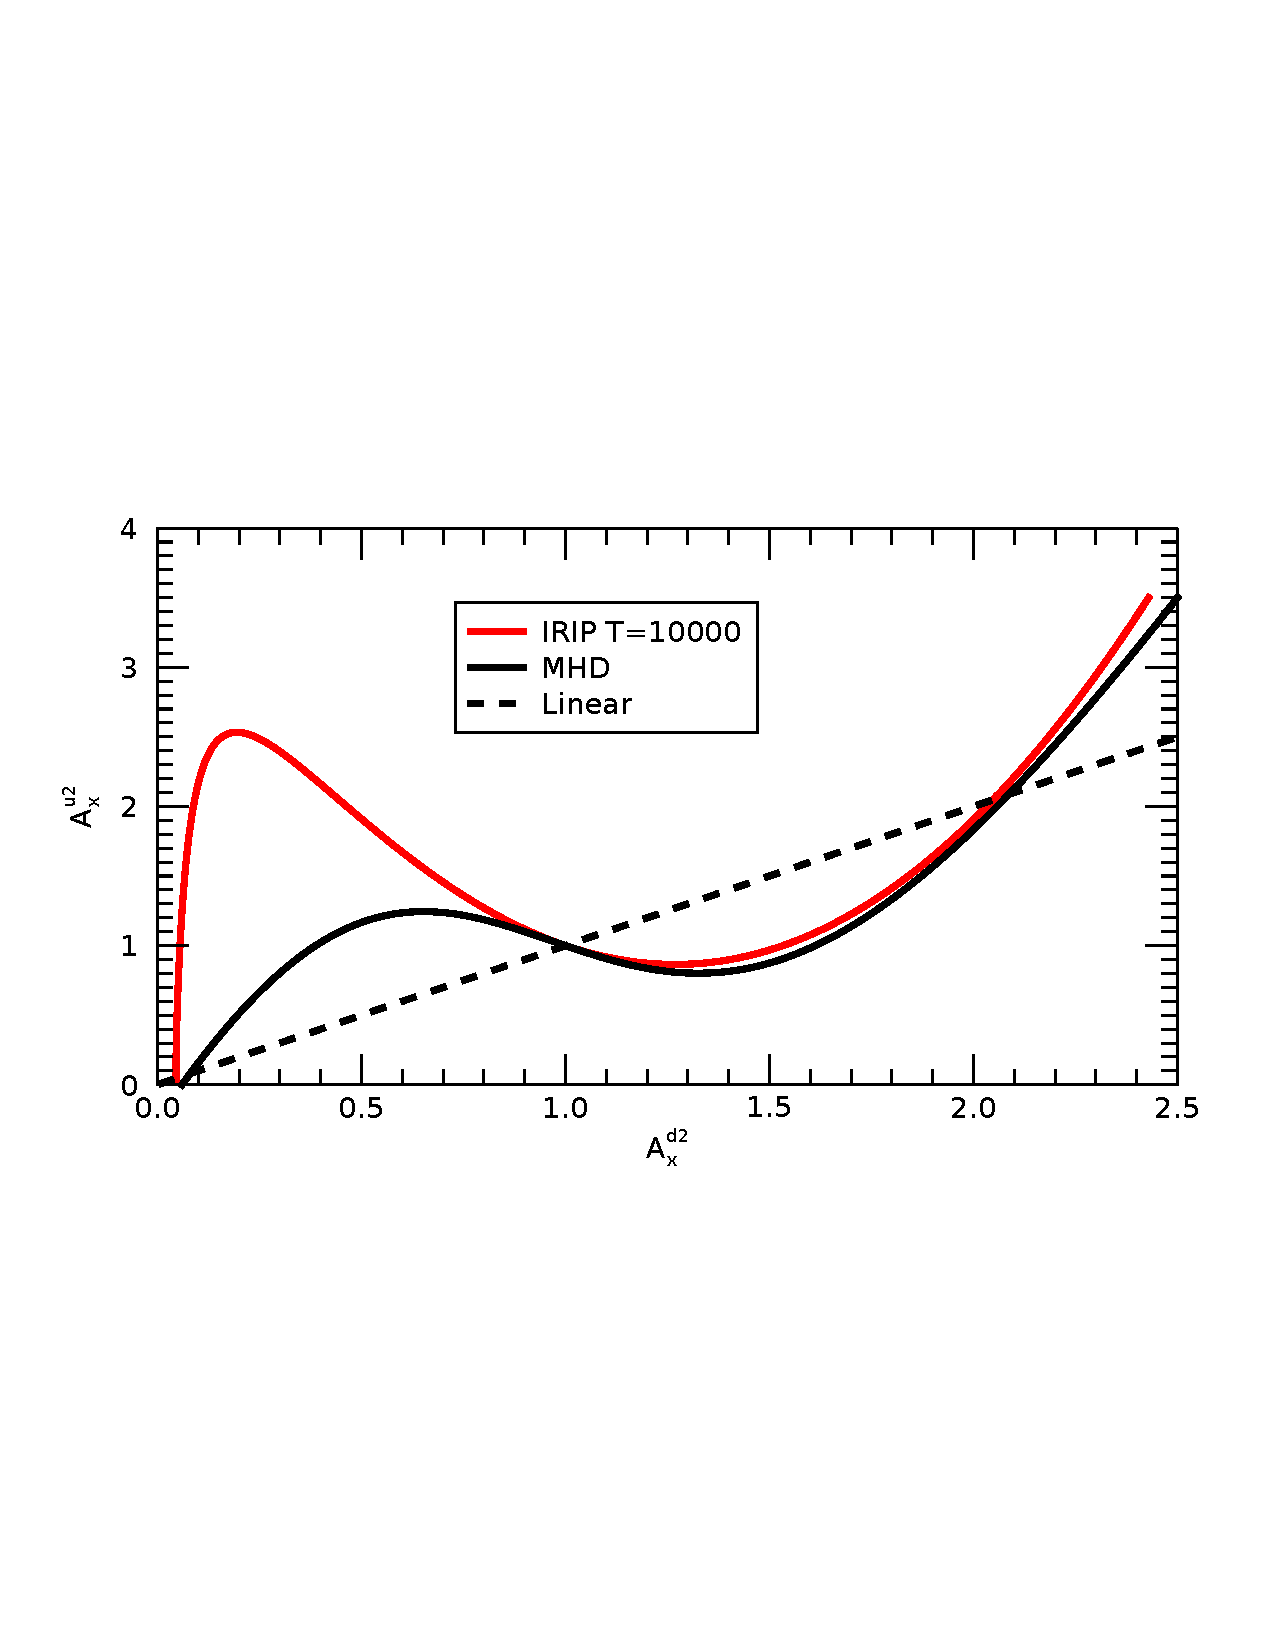
\includegraphics[width=0.9\linewidth,clip=true,trim=1.0cm 8.2cm 1.2cm 8.3cm]{tjumpplotex.pdf}
%     \caption{Solutions to the shock jump equations for the IRIP (red) and MHD (black) equations relating the upstream ($^u$) and downstream ($^d$) Alfv\'en Mach numbers $A_x$. The trivial solution ($A_x^{d}=A_x^{u}$) exists for both sets of equations. The parameters used for this plot are $T_0 = 10000$ K, $\beta = 0.1$, $\theta =\pi/4$ and $\gamma =5/3$.}
%     \label{fig:tjumpex}
% \end{figure}
% \end{column}
% \end{columns}
% \end{frame}

\begin{frame}{Equilibrium conditions - IRIP model}
\textbf{Ionisation, recombination and ionisation potential equilibrium conditions}
\begin{columns}
\begin{column}{0.45\textwidth}
\begin{figure}
    \centering
    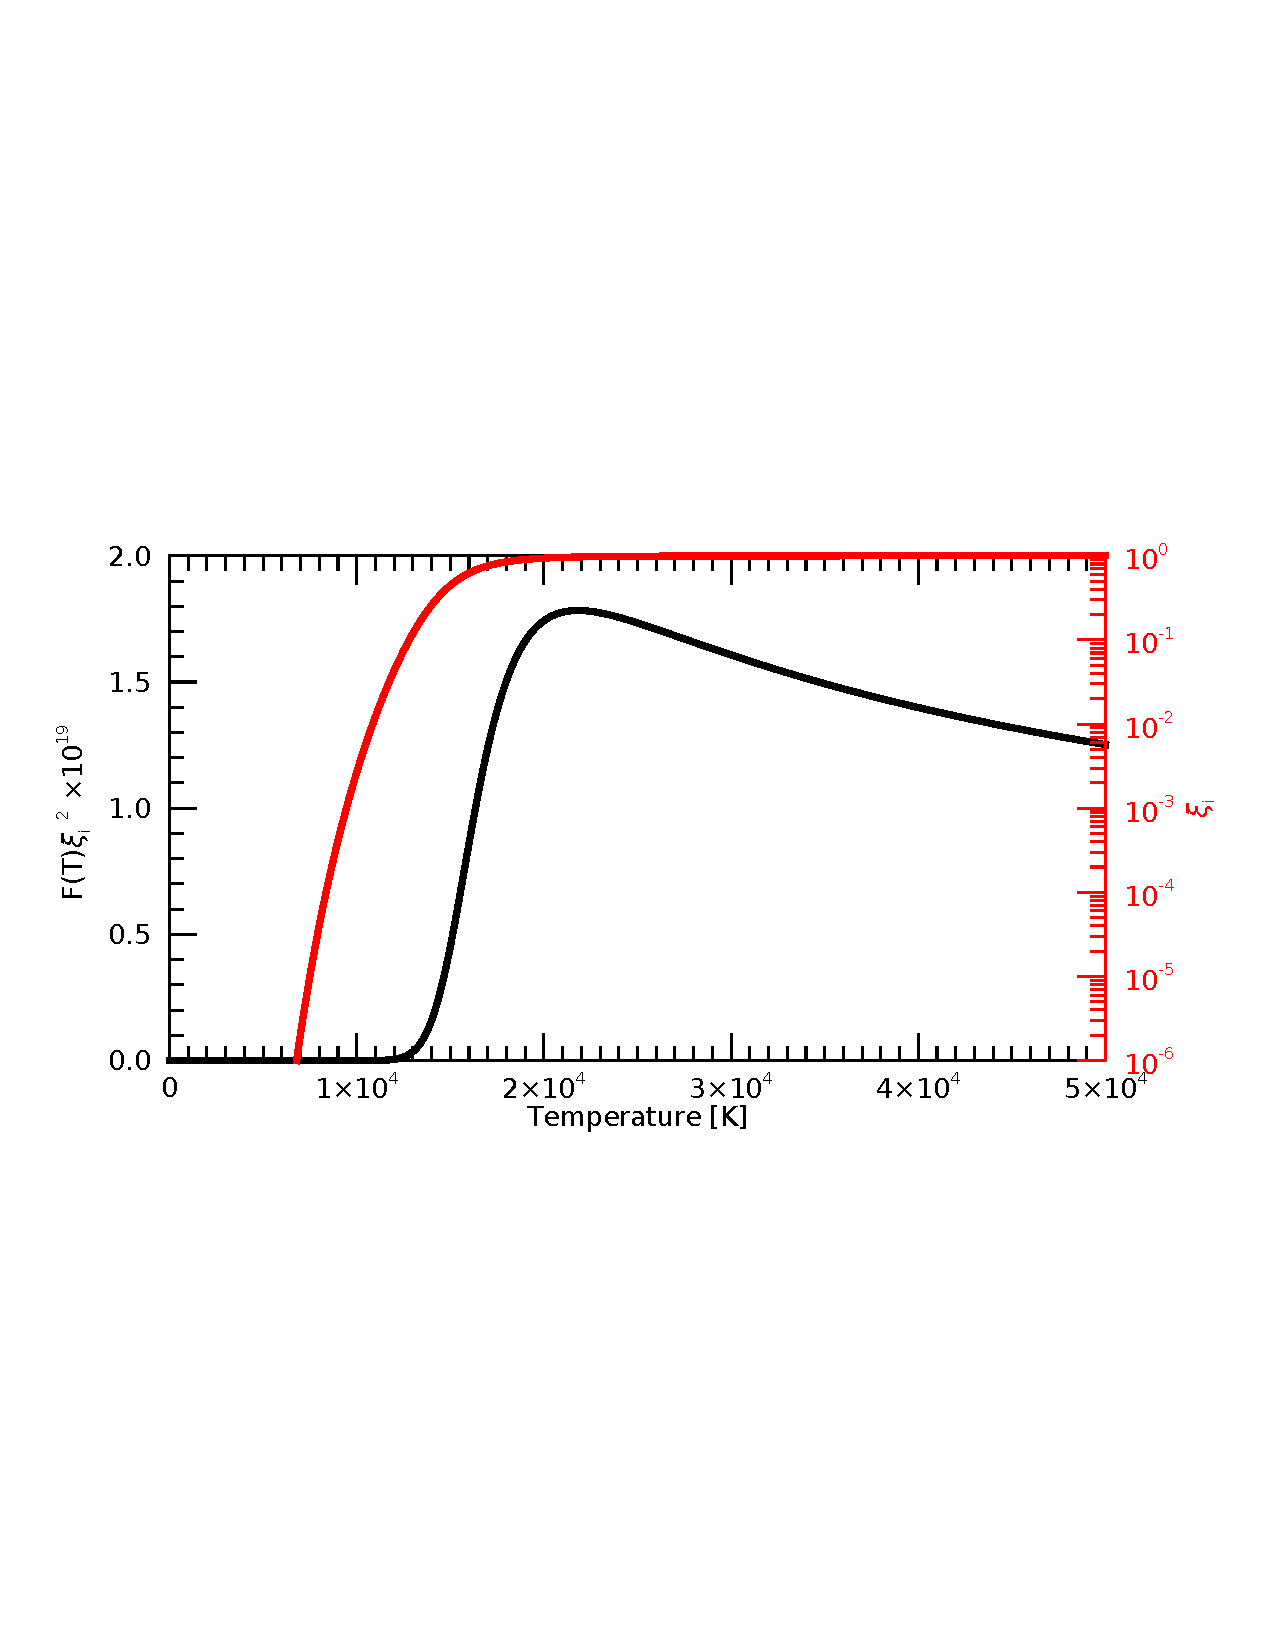
\includegraphics[width=0.95\linewidth,clip=true,trim=0.9cm 8.8cm 0.9cm 8.8cm]{Figures/eqltest3.pdf}
    \caption{$F(T) \xi_i^2$ as a function of temperature in dimensional form. Red line shows the ionisation fraction $\xi_i$ for the associated temperature.}
    \label{fig:eqltest}
\end{figure}
\end{column}
\begin{column}{0.55\textwidth}
Including the ionisation potential for an equilibrium, we require that the ionisation potential and heating terms balance:
\begin{gather}
    \hat{\phi} \Gamma _{ion} \rho_{\rm n} = \hat{\phi} \Gamma _{ion} (t=0) \rho _{\rm n} (t=0), \\
    \Gamma _{ion} \rho_{\rm n} = \Gamma _{rec} \rho_{\rm p} = \Gamma _{ion} (t=0) \rho _{\rm n} (t=0) =\mbox{const.} \\
    G(T)\rho_{\rm p} \rho_{\rm n} = F(T) \rho_{\rm p} ^2 = \mbox{const.} \\
    F(T) \xi_i ^2 \rho ^2 = \mbox{const.} \\
     \xi_i=\frac{1}{\frac{F(T)}{G(T)} +1}.
\end{gather}
\textbf{A compressible partially-ionised shock must cool across the interface!}
\end{column}
\end{columns}
\end{frame}

% \begin{frame}{Analytical solutions}
% \begin{columns}
% \begin{column}{0.4\textwidth}
% \begin{itemize}
% %\item Two-fluid model - ion+electron plasma, and bulk neutral fluid.
% \item Tricky terms are the heating and losses - non-conservative so need to know something about the underlying physics to determine
% \item Simplified empirical ionisation/recombination (used in most two-fluid solar codes)
% \item Analytically - simplified model implies shocks cool!
% \item Reduces to two coupled equations
% \end{itemize}
% \end{column}
% \begin{column}{0.6\textwidth}
% \end{column}
% \end{columns}
% \end{frame}

%%%%%%%%%%%%%%%%%%%%%%%%%%%%%%%%%%%%%%%%%

% \begin{frame}{Empirical collisional Ionisation/recombination model}
% \begin{columns}
% \begin{column}{0.3\textwidth}
% \begin{itemize}
% %\item Two-fluid model - ion+electron plasma, and bulk neutral fluid.
% \item Simplified empirical ionisation/recombination
% \item Analytically - simplified model implies shocks cool!
% \end{itemize}
% \end{column}
% \begin{column}{0.7\textwidth}
% \end{column}
% \end{columns}
% \end{frame}

% \begin{frame}{Similar effect in radiative coronal models?}
% \begin{columns}
% \begin{column}{0.3\textwidth}
% \begin{itemize}
% %\item Two-fluid model - ion+electron plasma, and bulk neutral fluid.
% \item Common to analyse coronal studies using constant heating term and empirical radiative loss function
% \item Solved in same way as before.
% \item Cooling shocks exist as a solution.
% \end{itemize}
% \end{column}
% \begin{column}{0.7\textwidth}
% \end{column}
% \end{columns}
% \end{frame}

\begin{frame}{Problems}
\begin{columns}
\begin{column}{0.5\textwidth}
\begin{itemize}
%\item Two-fluid model - ion+electron plasma, and bulk neutral fluid.
\item This implies shocks cool rather than heat! (Snow+2021)
\item Empirical rates are fitted to data warmer than the chromosphere
\item No radiation
\item All ionisation comes from ground state
\item Similar cooling solutions in corona-like radiative MHD model (Snow2023, in prep)  
\end{itemize}
\end{column}
\begin{column}{0.5\textwidth}
\begin{itemize}
%\item Two-fluid model - ion+electron plasma, and bulk neutral fluid.
\item Need more comprehensive model! Needs collisional and radiative rates. Self-consistent heating terms, etc.... 
\item Developed multi-level hydrogen model - offers unparalleled treatment of partial ionisation. 
\item Paper under review (Snow+2023b,MNRAS)
\end{itemize}
\end{column}
\end{columns}
\end{frame}

%%%%%%%%%%%%%%%%%%%%%%%%%%%%%%%%%%%%%%%%%%%%%%%%%%%%%%%%%%%%%%%
\begin{frame}{Ionisation/recombination model}
\begin{columns}
\begin{column}{0.3\textwidth}
\begin{itemize}
%\item Two-fluid model - ion+electron plasma, and bulk neutral fluid.
\item 5 levels of neutral hydrogen + continuum/ionised plasma.
\item Assume all neutral hydrogen levels move as one.
\item Optically thick approximation for Lyman transitions.
\item Leenaarts+2007, Johnson1972, Sollum1999
\end{itemize}
\end{column}
\begin{column}{0.7\textwidth}
\begin{gather}
    % \Gamma_{\rm rec} \rho_{\rm p} = \rho_{\rm p} (C_{\rm{p},1}+C_{\rm{p},2}+C_{\rm{p},3}+C_{\rm{p},4}+C_{\rm{p},5}) \nonumber \\
    %     \hspace{2cm}+ \rho_{\rm{p}} (R_{\rm{p},1}+R_{\rm{p},2}+R_{\rm{p},3}+R_{\rm{p},4}+R_{\rm{p},5}) \\
    %     \hspace{1.4cm} = \rho_p \Gamma_{\rm rec,c} + \rho_p \Gamma_{\rm rec,r}
    \Gamma_{\rm rec} \rho_{\rm p} = \rho_{\rm p} (\hat{C}_{\rm{p},1}+\hat{C}_{\rm{p},2}+\hat{C}_{\rm{p},3}+\hat{C}_{\rm{p},4}+\hat{C}_{\rm{p},5})/\hat{\Gamma} \nonumber \\
        \hspace{1.2cm}+ \rho_{\rm{p}} (\hat{R}_{\rm{p},1}+\hat{R}_{\rm{p},2}+\hat{R}_{\rm{p},3}+\hat{R}_{\rm{p},4}+\hat{R}_{\rm{p},5})/\hat{\Gamma} \nonumber \\
        \hspace{1.2cm} = \rho_{\rm p} (\hat{\Gamma}_{\rm rec,col} + \hat{\Gamma}_{\rm rec,rec})/\hat{\Gamma} \nonumber
\end{gather}
\begin{gather}
    \Gamma_{\rm ion} \rho_{\rm{n}} = (\rho_{\rm{n}1} \hat{C}_{1,\rm{p}}+\rho_{n2}\hat{C}_{2,\rm{p}}+\rho_{\rm{n}3}\hat{C}_{3,\rm{p}}+\rho_{\rm{n}4}\hat{C}_{4,\rm{p}}+\rho_{\rm{n}5}\hat{C}_{5,\rm{p}})/\hat{\Gamma} \nonumber \\  
    \hspace{1cm}+(\rho_{\rm{n}1}\hat{R}_{1,\rm{p}}+\rho_{\rm{n}2}\hat{R}_{2,\rm{p}}+\rho_{\rm{n}3} \hat{R}_{3,\rm{p}}+\rho_{\rm{n}4}\hat{R}_{4,\rm{p}}+\rho_{\rm{n}5}\hat{R}_{5,\rm{p}})/\hat{\Gamma}  \nonumber\\
    \hspace{1cm} = \rho_{\rm{n}} (\hat{\Gamma}_{\rm ion,col} + \hat{\Gamma}_{\rm ion,rad})/\hat{\Gamma} \nonumber
\end{gather}
Rate coefficients $C,R$ are functions of temperature and electron number density 
\end{column}
\end{columns}
\end{frame}


\begin{frame}{Numerical model}
\begin{columns}
\begin{column}{0.5\textwidth}
\begin{enumerate}
\item 1D shocks in two-fluid partially-ionised plasma using (P\underline{I}P) code.
\item Investigate shock substructure.
\item Initial conditions produce switch-off slow-mode shock.
\item Initial level populations determined by reference electron number density and temperature
\item Equilibrium recombination timescale set to $10^{-5}$ of collisional timestep.
\item 512000 grid cells, 1st order HLLD solver, explicit integration of source terms.
\end{enumerate}
\end{column}
\begin{column}{0.5\textwidth}
\begin{eqnarray}
B_x &=& 0.1  \nonumber\\
B_y &=& -1.0 (x>0), 1.0 (x<0) \nonumber \\
\rho _n &=& \xi _n \rho _{tot} \nonumber \\
\rho _p &=& \xi _i \rho _{tot} = (1- \xi _n) \rho _{tot} \nonumber \\
P_n &=& \frac{\xi _n}{\xi_n + 2 \xi _i} P_{tot} =  \frac{\xi _n}{\xi_n + 2 \xi _i} \beta \frac{B_0 ^2}{2} \nonumber \\
P_p &=& \frac{2 \xi _i}{\xi_n + 2 \xi _i} P_{tot} =  \frac{2 \xi _i}{\xi_n + 2 \xi _i} \beta \frac{B_0 ^2}{2} \nonumber
\end{eqnarray}
\end{column}
\end{columns}
\end{frame}

\begin{frame}{Numerical simulation - mid chromosphere}
\begin{columns}
\begin{column}{0.8\textwidth}
\begin{figure}
    %\centering
    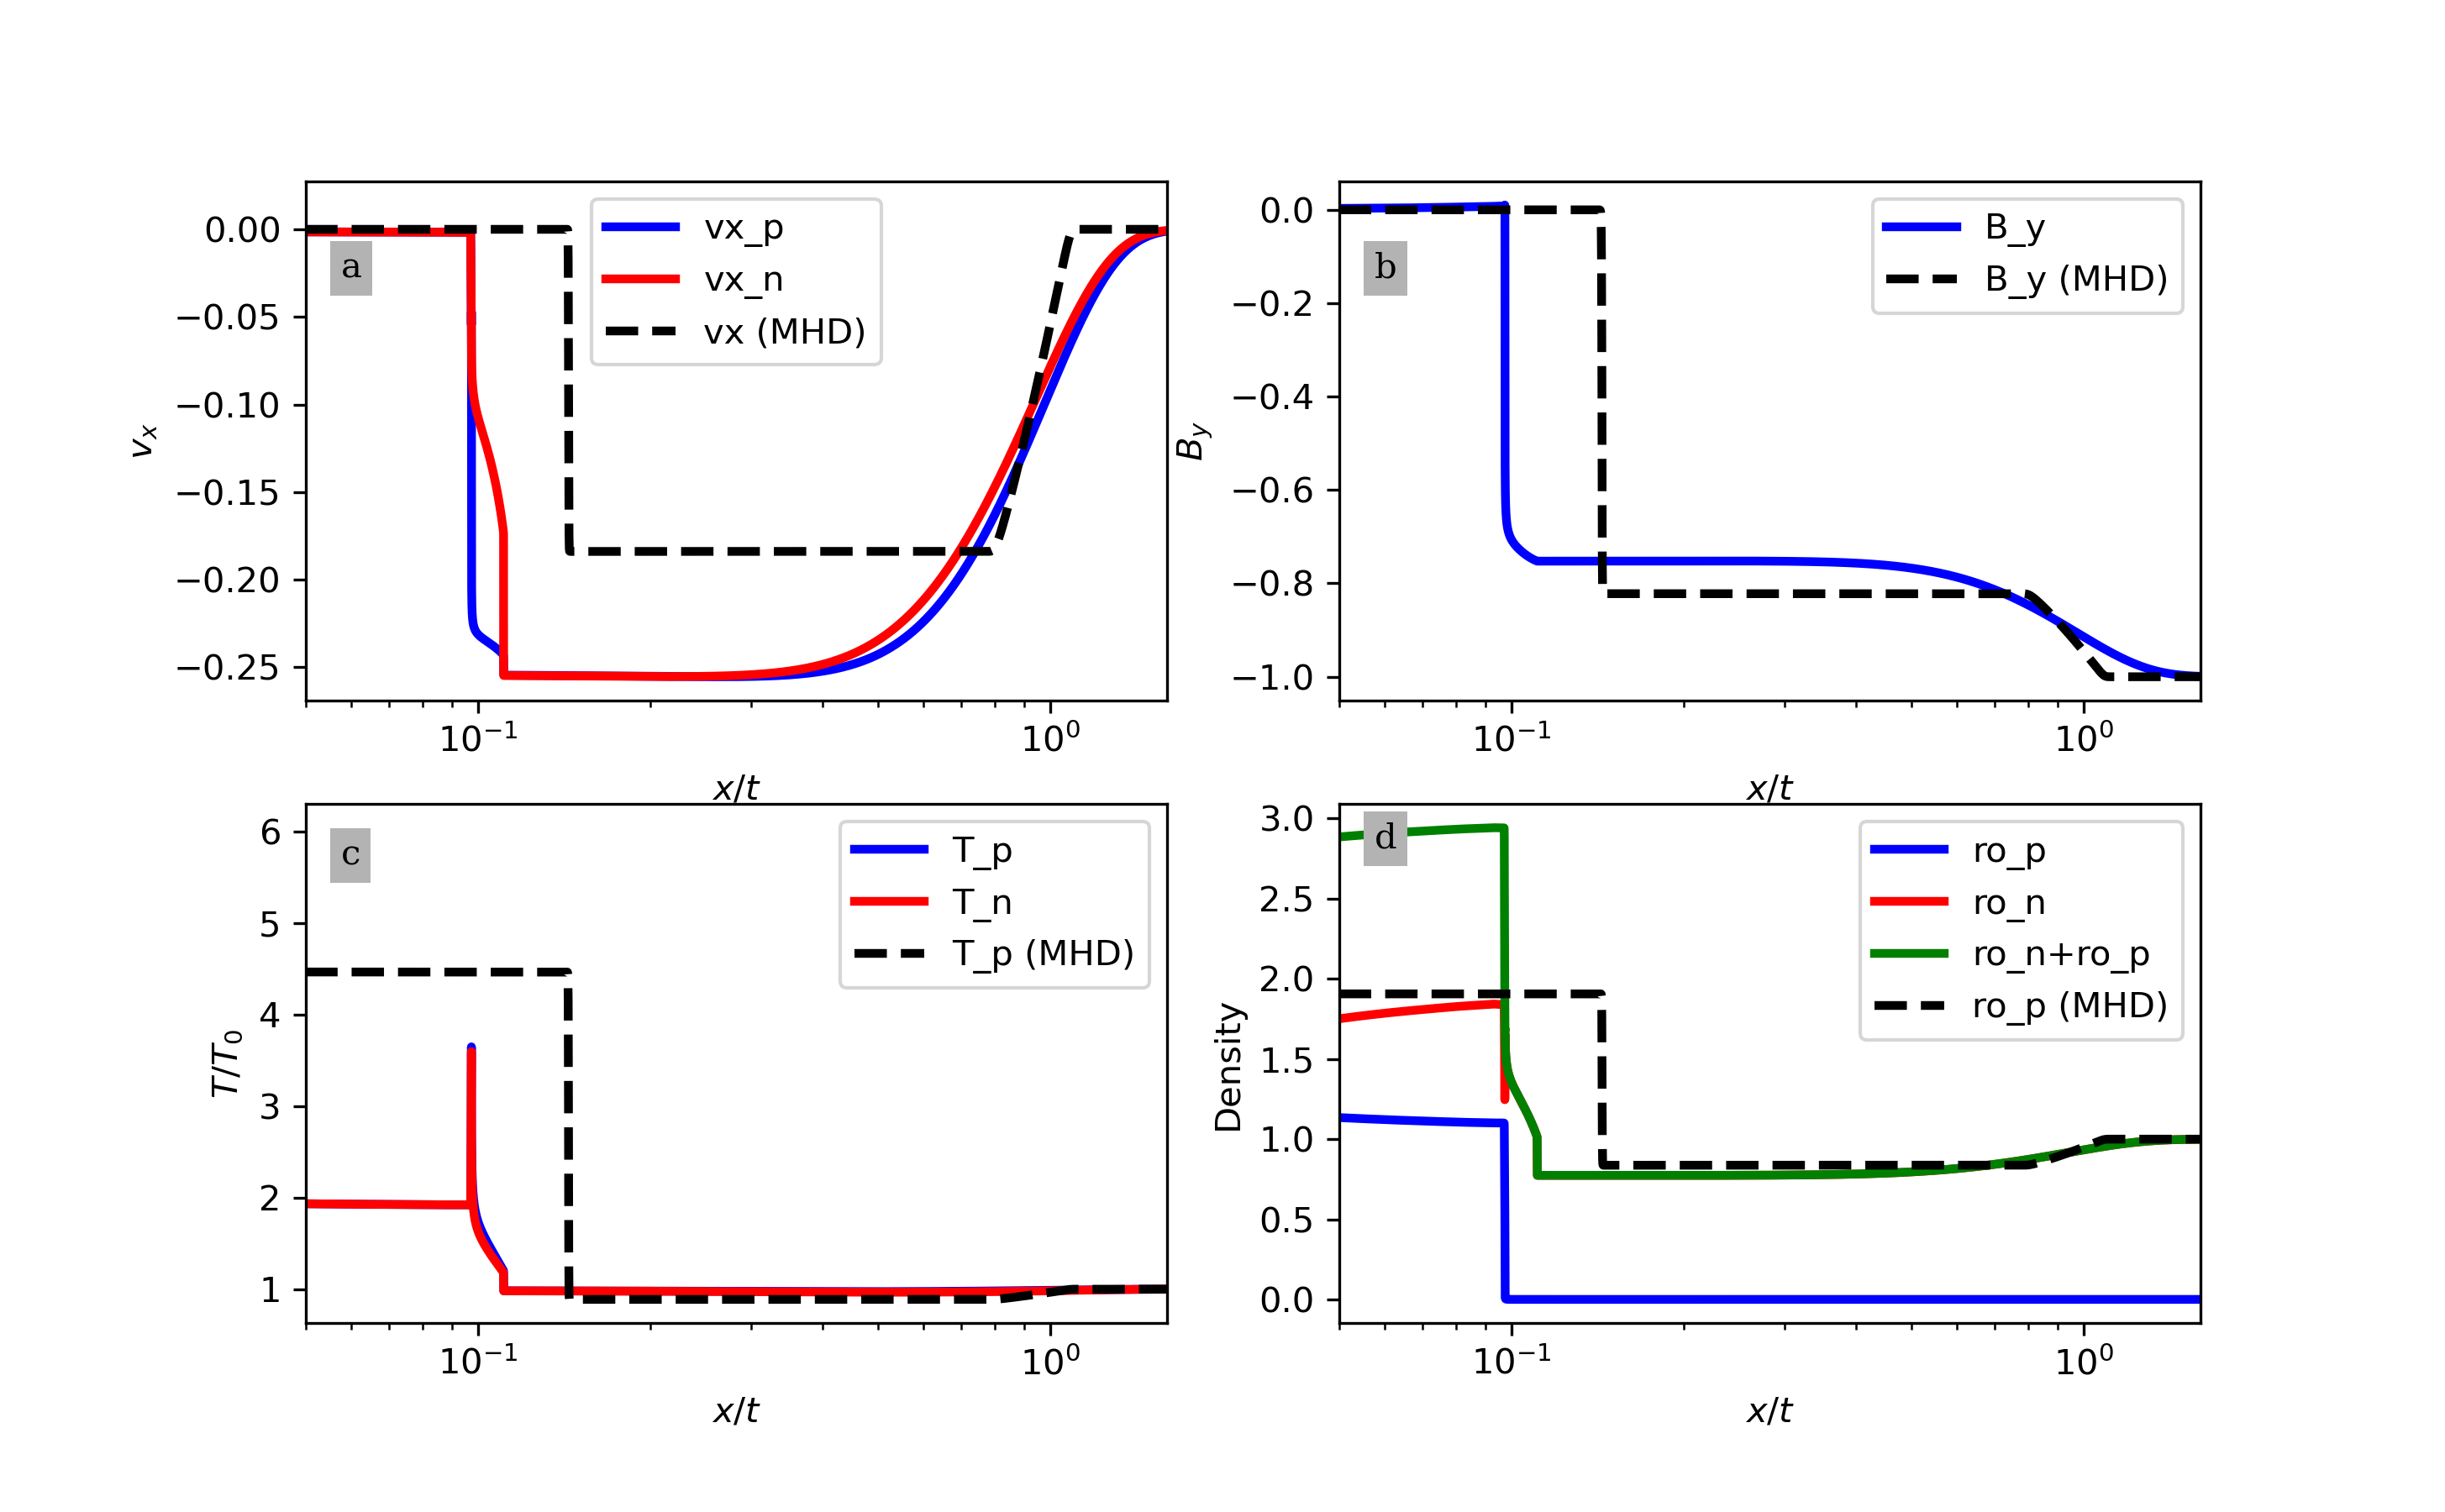
\includegraphics[width=0.95\linewidth,clip=true,trim=0.9cm 0.8cm 0.9cm 0.8cm]{2023StAndrews/Figures/context_midc_corrected.png}
    %\caption{Upper-chromosphere case showing the $v_x$ velocity (top left), $B_y$ magnetic field (top right), temperature (lower left) and density (lower right). For panel c, the reference temperature $T_0=6220$.}
    \label{fig:upperchromocontext}
\end{figure}
\end{column}
\begin{column}{0.2\textwidth}
%\begin{itemize}
    $T_0=5030$, $n_e=7.5\times 10^{16}$, $\xi_n=0.9997$
%\end{itemize}
\end{column}
\end{columns}
\end{frame}

% \begin{frame}{Shock substructure - mid chromosphere}
% \begin{columns}
% \begin{column}{0.8\textwidth}
% \begin{figure}
%     %\centering
%     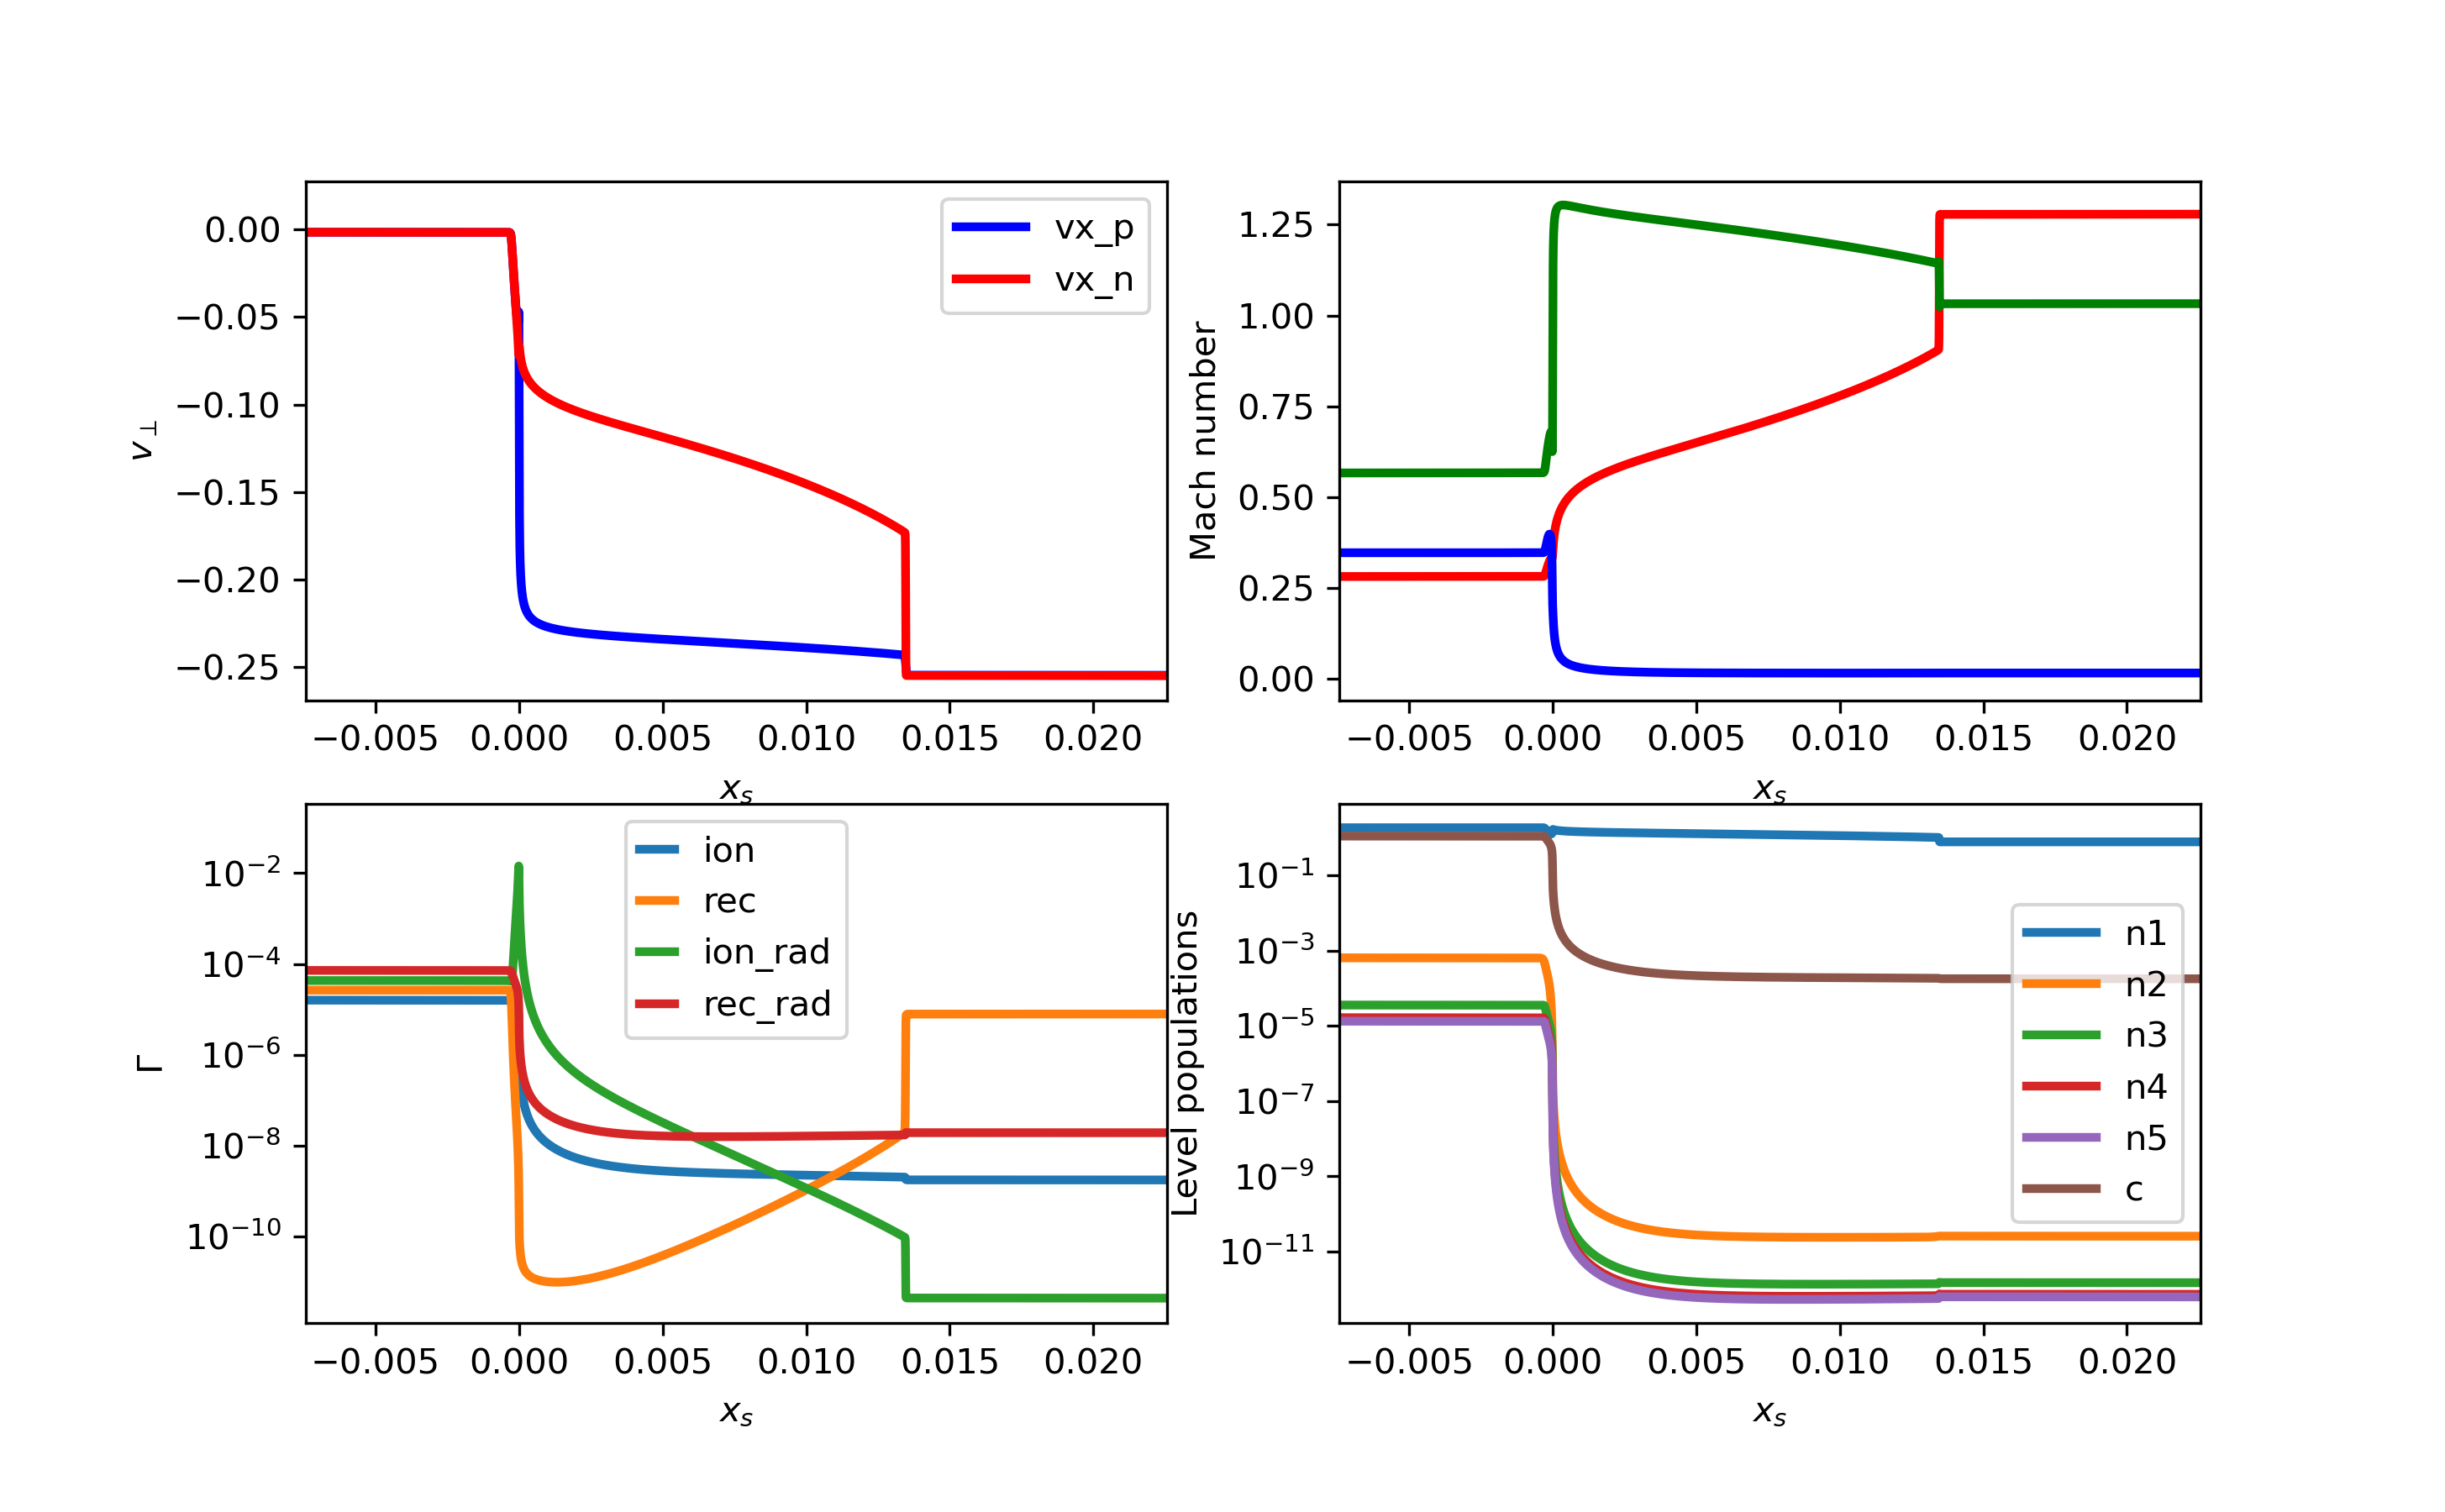
\includegraphics[width=0.95\linewidth,clip=true,trim=1.2cm 0.8cm 0.9cm 0.8cm]{2023StAndrews/Figures/shocksub2_plot_midc_corrected.png}
%     %\caption{Upper-chromosphere case showing the $v_x$ velocity (top left), $B_y$ magnetic field (top right), temperature (lower left) and density (lower right). For panel c, the reference temperature $T_0=6220$.}
%     \label{fig:upperchromocontext}
% \end{figure}
% \end{column}
% \begin{column}{0.2\textwidth}
% %\begin{itemize}
%     $T_0=5030$, $n_e=7.5\times 10^{16}$, $\xi_n=0.9997$
% %\end{itemize}
% \end{column}
% \end{columns}
% \end{frame}


\begin{frame}{Cooling through the shock}
\begin{columns}
\begin{column}{0.5\textwidth}
\begin{figure}
    \centering
    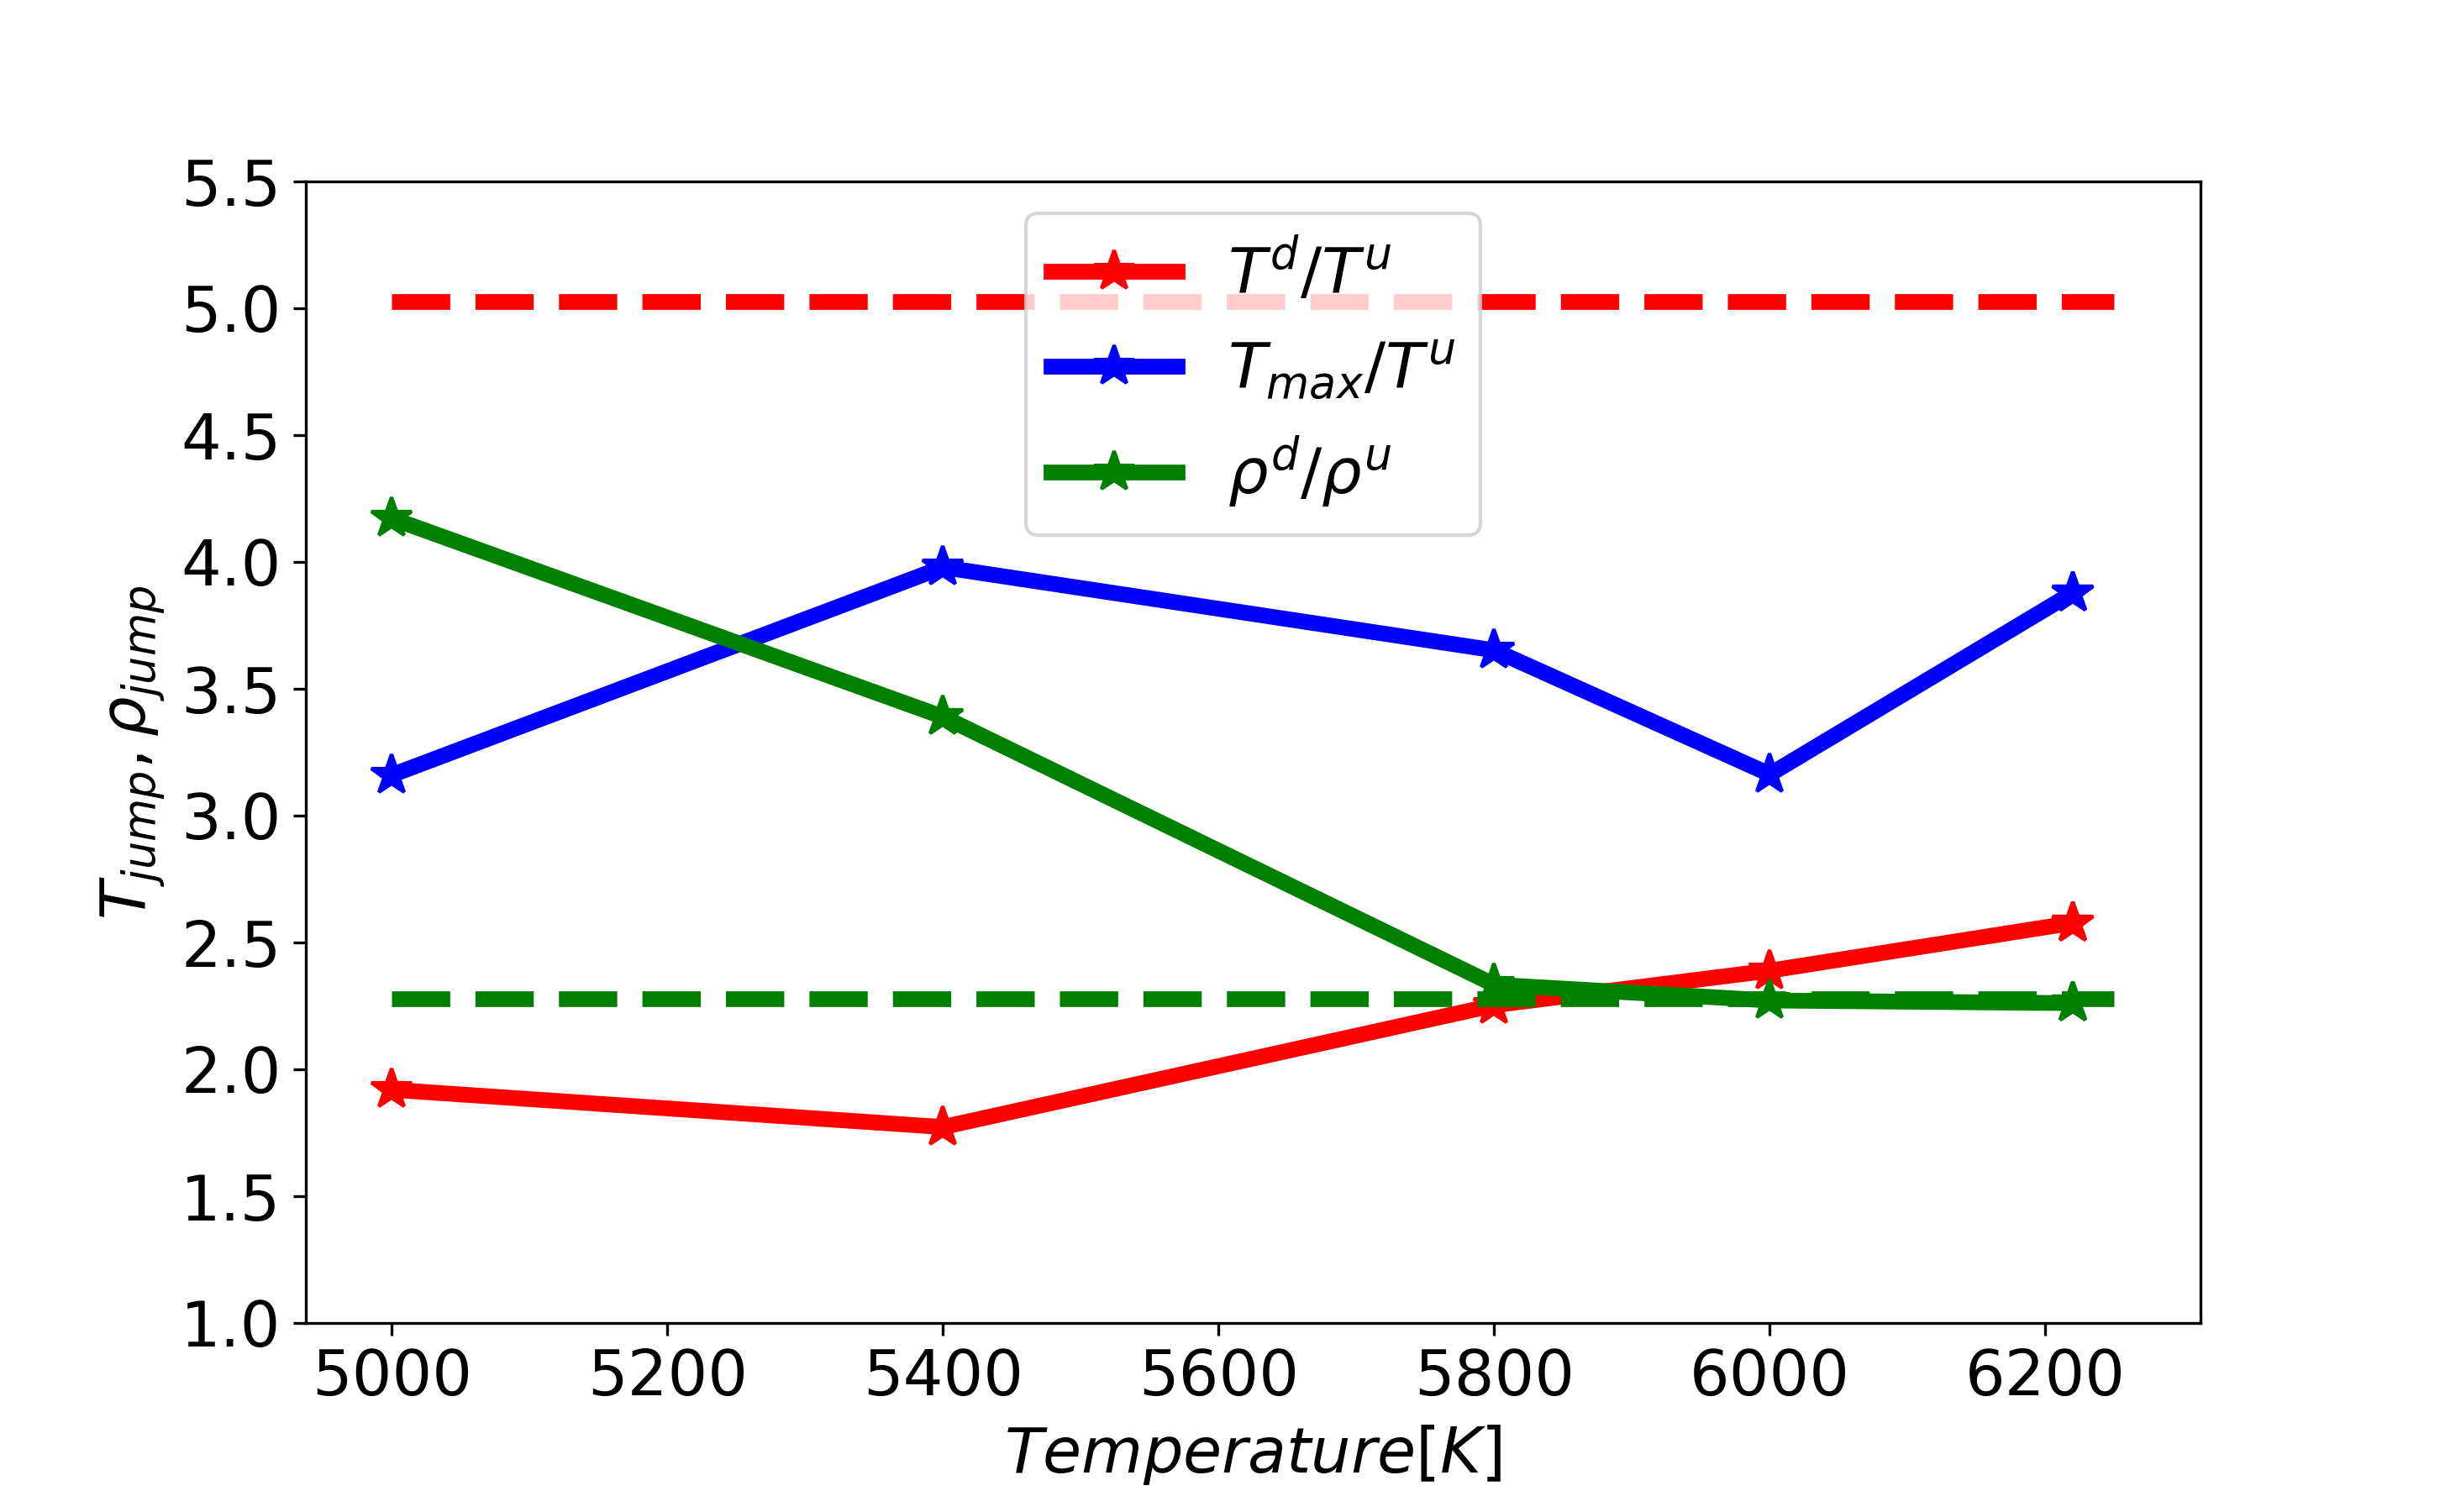
\includegraphics[width=0.95\linewidth,clip=true,trim=1.2cm 0.3cm 1.6cm 1.8cm]{2023StAndrews/Figures/tcompcor_plot.png} \\
    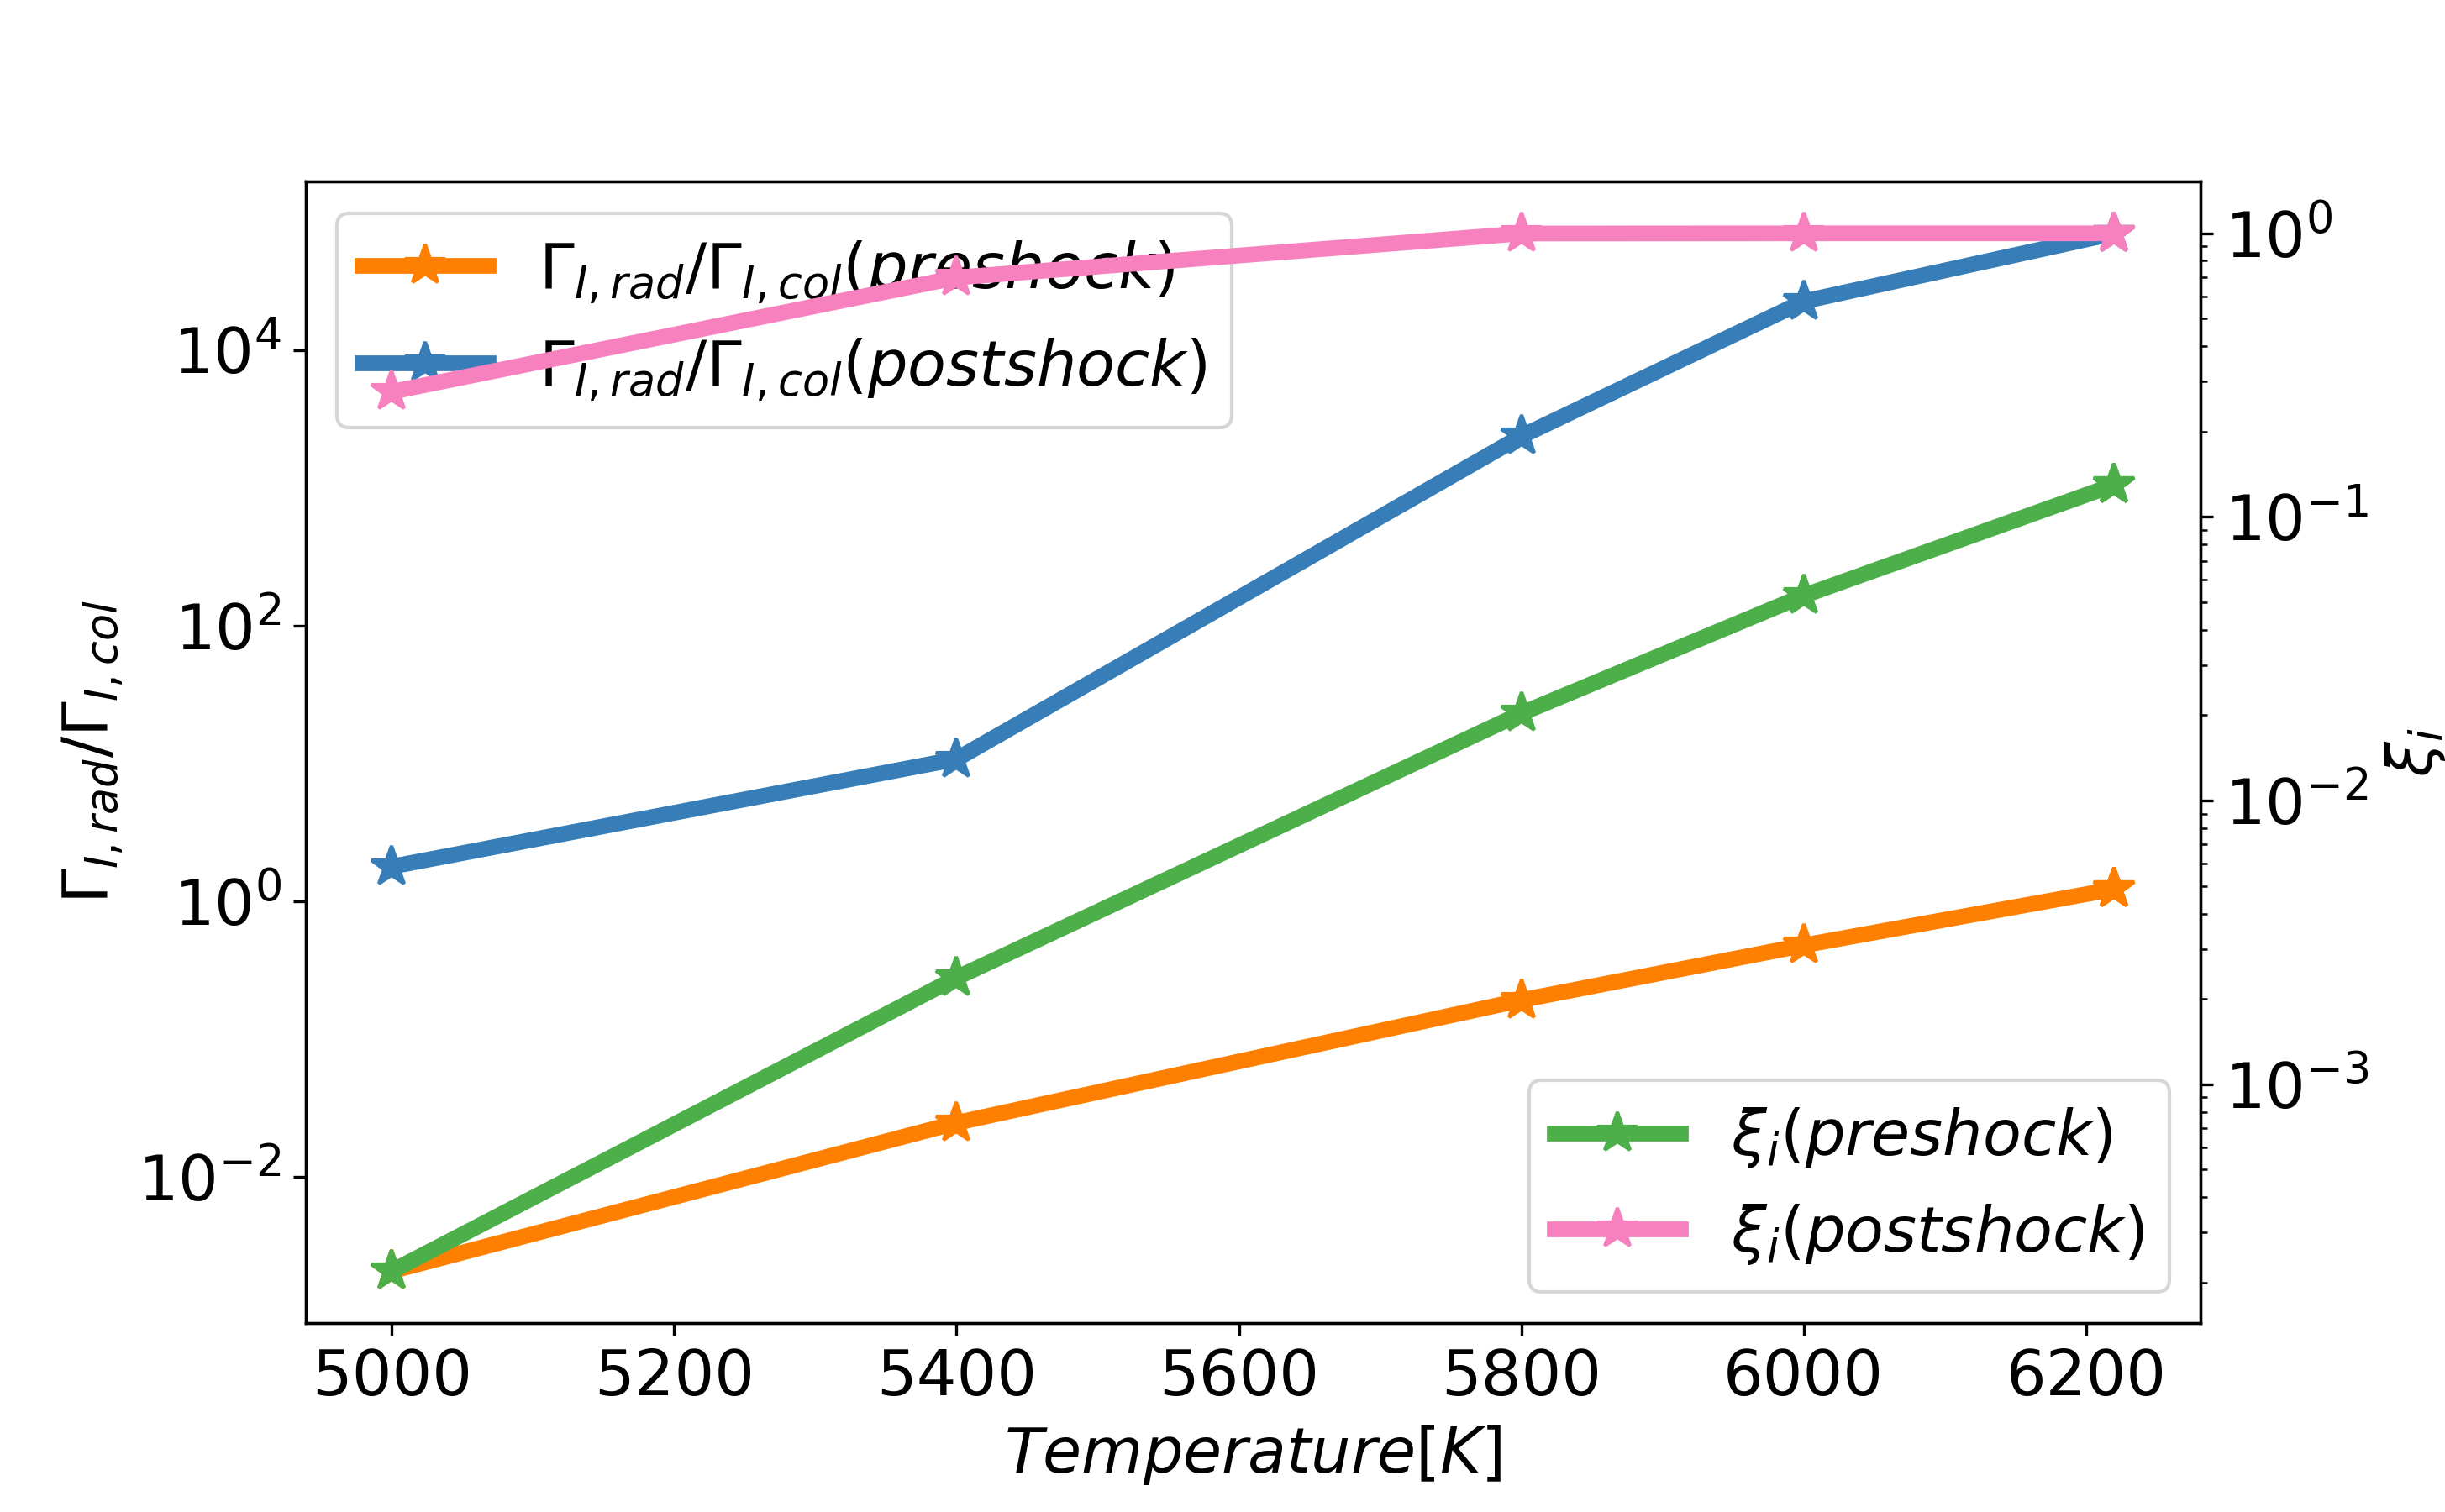
\includegraphics[width=0.95\linewidth,clip=true,trim=0.4cm 0.3cm 0.1cm 1.8cm]{2023StAndrews/Figures/tcompcor_ion_plot.png}
\end{figure}
\end{column}
\begin{column}{0.42\textwidth}
\begin{itemize}
    \item Constant reference electron number density
    \item Temperature increase much less than predicted by MHD
    \item Density increase much greater than MHD
    \item Rankine-Hugoniot jump conditions (based on ideal MHD) may not apply to lower atmosphere shocks - dissipation estimates incorrect? (Anan+2019)
    \item DKIST observation of umbral flashes shows density jump $\approx 3.82$ for slow-mode shock (French+2023) 
    %\item Observational consequences - flares?
\end{itemize}
\end{column}
\end{columns}
\end{frame}


% \begin{frame}{Conclusions}
% \begin{itemize}
%     \item Non-equilibrium ionisation fundamentally changes the behaviour of shocks.
%     \item Temperature jump across the shock is significantly cooler than the MHD value.
%     \item Maximum temperature within the shock also cooler.
%     \item Density increase far greater than MHD.
%     \item Rankine-Hugoniot jump conditions may not apply to lower atmosphere shocks.
%     \item How would this affect observations?
% \end{itemize}
% \end{frame}

% \begin{frame}{Research excellence}
% \begin{itemize}
%     \item Leading expert in partial ionisation
%     \item Developed open-source tools - (PIP), shockID
%     \item Strong publication record
%     \item 
% \end{itemize}
% \end{frame}

\begin{frame}{Vision for the future}
\begin{itemize}
    \item Open question about the role of shocks in heating - \textbf{do they cool or heat the plasma, and by how much?}
    \item Theory requires ground-up rewrite.
    \item Semi-analytical solutions possible (Snow+2021).
    \item Need to study larger systems - turbulent reconnection, shocks in sunspots
    \item Connect the theory to observations via numerical simulations and optically thick forward modelling.
    %\item Research proposals well developed.
    \item Funding proposals: Leverhulme Research Project Grant, ERC Starting Grant, Future Leaders Fellowship. 
\end{itemize}
\end{frame}

%%%%%%%%%%%%%%%%%%%%%%%%%%%%%%%%%%%%%%%%%%%%%%%%%%%%%%%%%%%%%%%%

% \begin{frame}{Populations at different heights}
% \begin{columns}
% \begin{column}{0.5\textwidth}
% \begin{figure}
%     \centering
% %\includegraphics[width=0.95\linewidth,clip=true,trim=0.9cm 7.8cm 1.5cm 7.8cm]{figures/widthradt2_sw.pdf}
% %    \caption{Finite width of the shock as a function of upstream recombination rates.}
%     \includegraphics[width=0.95\linewidth]{2023RAS/Figures/saha2_plot.png}
%     \caption{Temperature (red) and ion fraction through height (using VALCIII data)}
%     \label{fig:shockwidthsw}
% \end{figure}
% \end{column}
% \begin{column}{0.42\textwidth}
% \begin{itemize}
%     \item Different atmospheric heights have different temperatures and electron number densities.
%     \item Different importance of radiative/collisional rates
%     \item Sample a few heights
% \end{itemize}
% \end{column}
% \end{columns}
% \end{frame}

% \begin{frame}{Numerical simulation - mid chromosphere}
% \begin{columns}
% \begin{column}{0.8\textwidth}
% \begin{figure}
%     %\centering
%     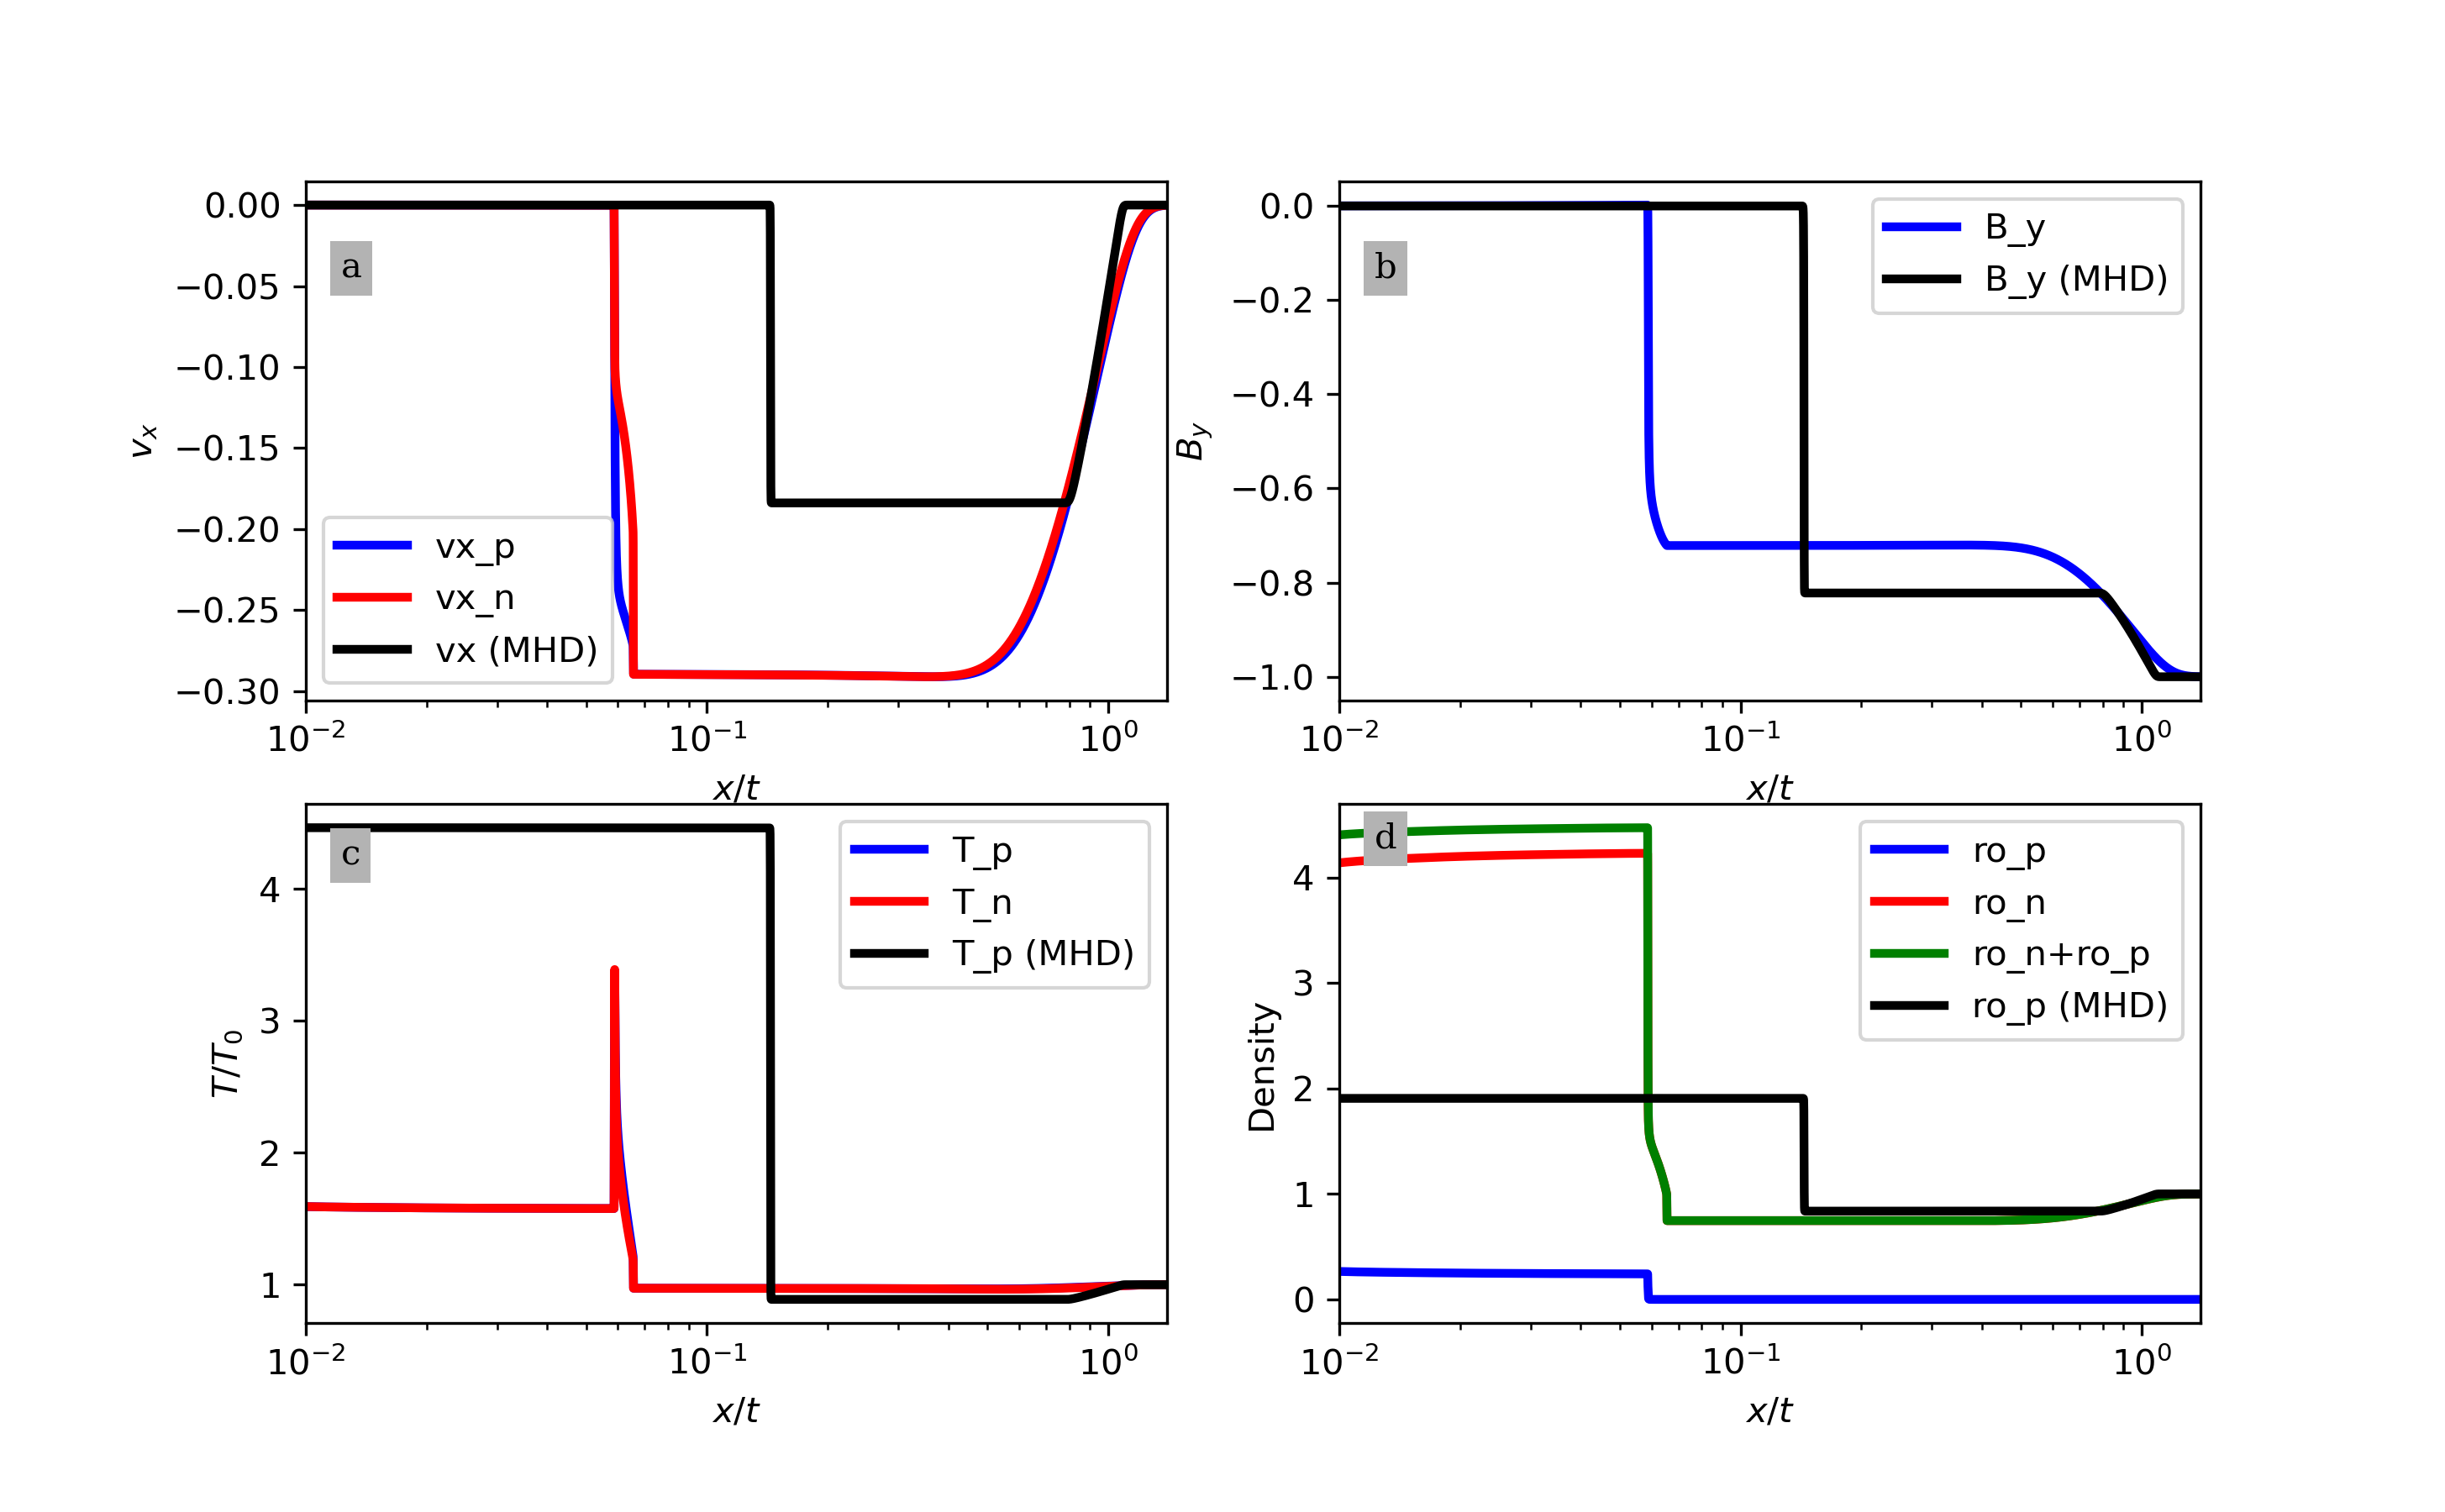
\includegraphics[width=0.95\linewidth,clip=true,trim=0.9cm 0.8cm 0.9cm 0.8cm]{2023RAS/Figures/context_midc.png}
%     %\caption{Upper-chromosphere case showing the $v_x$ velocity (top left), $B_y$ magnetic field (top right), temperature (lower left) and density (lower right). For panel c, the reference temperature $T_0=6220$.}
%     \label{fig:midchromocontext}
% \end{figure}
% \end{column}
% \begin{column}{0.2\textwidth}
% %\begin{itemize}
%     $T_0=5030$, $n_e=7.5\times 10^{16}$, $\xi_n=0.9997$
% %\end{itemize}
% \end{column}
% \end{columns}
% \end{frame}

% \begin{frame}{Shock substructure - mid chromosphere}
% \begin{columns}
% \begin{column}{0.8\textwidth}
% \begin{figure}
%     %\centering
%     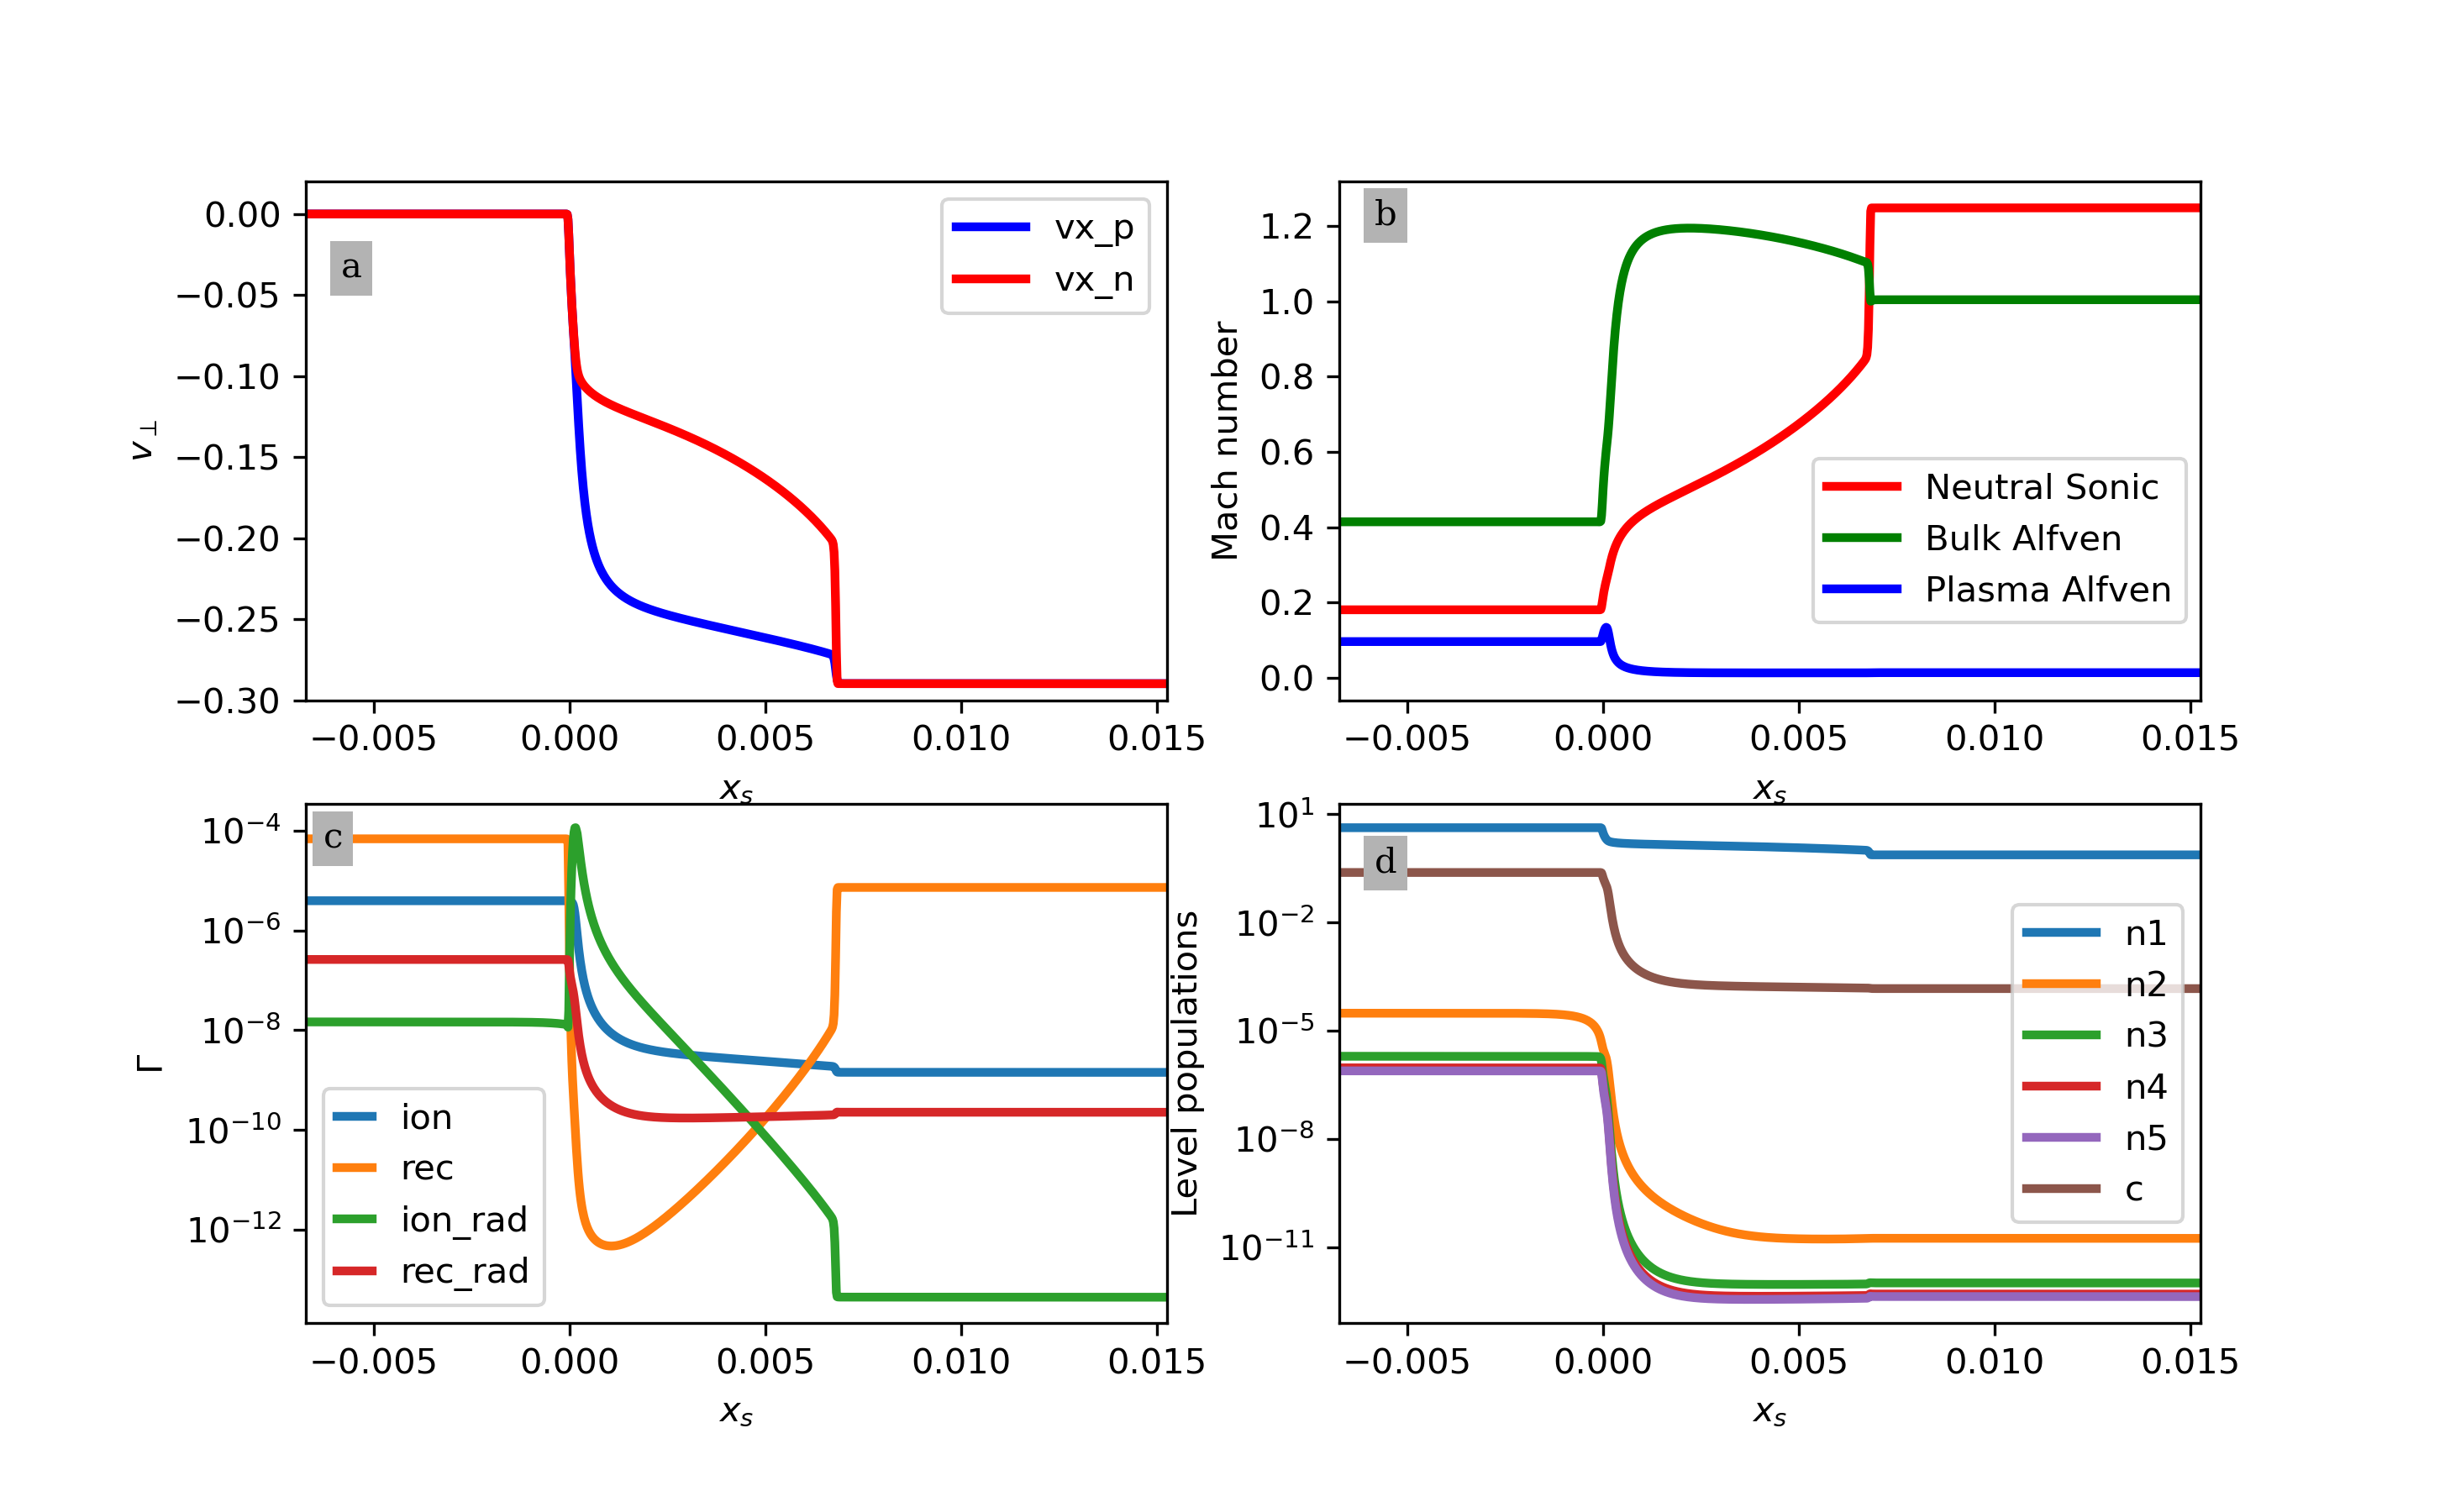
\includegraphics[width=0.9\linewidth,clip=true,trim=1.2cm 0.8cm 0.9cm 0.8cm]{2023RAS/Figures/shocksub2_plot_midc.png}
%     %\caption{Upper-chromosphere case showing the $v_x$ velocity (top left), $B_y$ magnetic field (top right), temperature (lower left) and density (lower right). For panel c, the reference temperature $T_0=6220$.}
%     \label{fig:midchromocontext}
% \end{figure}
% \end{column}
% \begin{column}{0.2\textwidth}
% %\begin{itemize}
%     $T_0=5030$, $n_e=7.5\times 10^{16}$, $\xi_n=0.9997$
% %\end{itemize}
% \end{column}
% \end{columns}
% \end{frame}

\end{document}
